\chapter{Contributo Personale}\label{chapter:implementazioni}
La ristrutturazione del gestionale ha visto un intervento che si è concentrato prevalentemente sull'area relativa alla gestione dei clienti. In particolare, sono state apportate diverse modifiche e miglioramenti per ottimizzare il flusso di lavoro e la gestione delle informazioni.

Un aspetto chiave delle modifiche riguarda l'espansione delle funzionalità esistenti per consentire una gestione più dettagliata e completa dei dati relativi ai clienti. Tra le principali novità, sono state introdotte nuove sezioni che permettono di monitorare e gestire con maggiore precisione:
\begin{itemize}
    \item \textbf{Leads:} per tracciare le opportunità di vendita e monitorare l'avanzamento di ogni potenziale cliente.
    \item \textbf{Appuntamenti:} per organizzare e tenere traccia degli incontri e delle interazioni con i clienti.
    \item \textbf{Offerte:} per gestire le proposte commerciali e monitorarne lo stato di avanzamento.
    \item \textbf{Task:} per la gestione delle attività associate a ciascun cliente, migliorando l'assegnazione e il monitoraggio delle azioni da intraprendere.
\end{itemize}
Questi miglioramenti hanno reso il gestionale più versatile, consentendo agli utenti di avere una visione più completa e aggiornata delle attività legate ai propri clienti. L'introduzione di queste sezioni ha contribuito a migliorare l'efficienza operativa, facilitando la pianificazione e l'esecuzione delle attività quotidiane.
\pagebreak
\section{Prima e ora}\label{sec:cap_sec_subsec_prima_e_ora}
Prima delle modifiche introdotte, la gestione dei clienti nel sistema risultava piuttosto semplice e centralizzata. Ogni cliente veniva trattato come un'entità unica, senza una distinzione tra i diversi stadi del processo di acquisizione o gestione. In pratica, i dati relativi ai clienti erano registrati e archiviati senza un livello di dettaglio che permettesse di tracciare l'evoluzione di un cliente dalla fase iniziale di interesse fino alla finalizzazione di un contratto o di un progetto.

Il sistema era strutturato per gestire unicamente le informazioni base dei clienti, come nome, contatti e dettagli generali. Non c'era una chiara separazione tra i clienti già acquisiti e i potenziali clienti, i cosiddetti \textit{Leads}, né una gestione dei task o delle offerte. Questo rendeva difficile monitorare lo stato di avanzamento delle trattative, con una gestione che si limitava a un archivio statico delle informazioni.

Le modifiche apportate hanno trasformato significativamente il modo in cui il sistema gestisce i clienti, rendendo il flusso di lavoro più dinamico e interattivo. In particolare, è stata introdotta una separazione tra i \textbf{Leads} e i clienti acquisiti. Ora, ogni potenziale cliente (Lead) può essere tracciato separatamente, permettendo una gestione più precisa e una visibilità migliore sullo stato delle trattative.

Le nuove funzionalità permettono di:
\begin{itemize}
    \item Monitorare i \textbf{Leads}, che rappresentano i potenziali clienti ancora nella fase di acquisizione.
    \item Gestire gli \textbf{Appuntamenti}, per programmare e tenere traccia delle interazioni con i clienti/leads.
    \item Creare e gestire \textbf{Offerte}, per monitorare le proposte fatte ai clienti/leads e il loro stato.
    \item Gestire i \textbf{Task} associati a ciascun cliente/lead, facilitando l'assegnazione e la pianificazione delle attività.
\end{itemize}
Queste modifiche hanno reso il sistema più fluido, con la possibilità di avere una visione completa delle opportunità di vendita e delle attività in corso. La divisione tra Leads e clienti acquisiti ha consentito una gestione più efficiente delle priorità e ha migliorato la pianificazione delle risorse. Di seguito la tabella visualizzata:

\section{Tabella dei Clienti e Leads}\label{sec:cap_sec_subsec_clienti_e_leads}
Per la gestione unificata di Clienti e Leads, è stata utilizzata una singola tabella nel database, distinguendo le due tipologie attraverso la colonna \texttt{is\_customer}. Questa colonna assume un valore booleano, dove \texttt{true} indica un Cliente e \texttt{false} identifica un Lead.

\begin{figure}[ht]
	\centering
	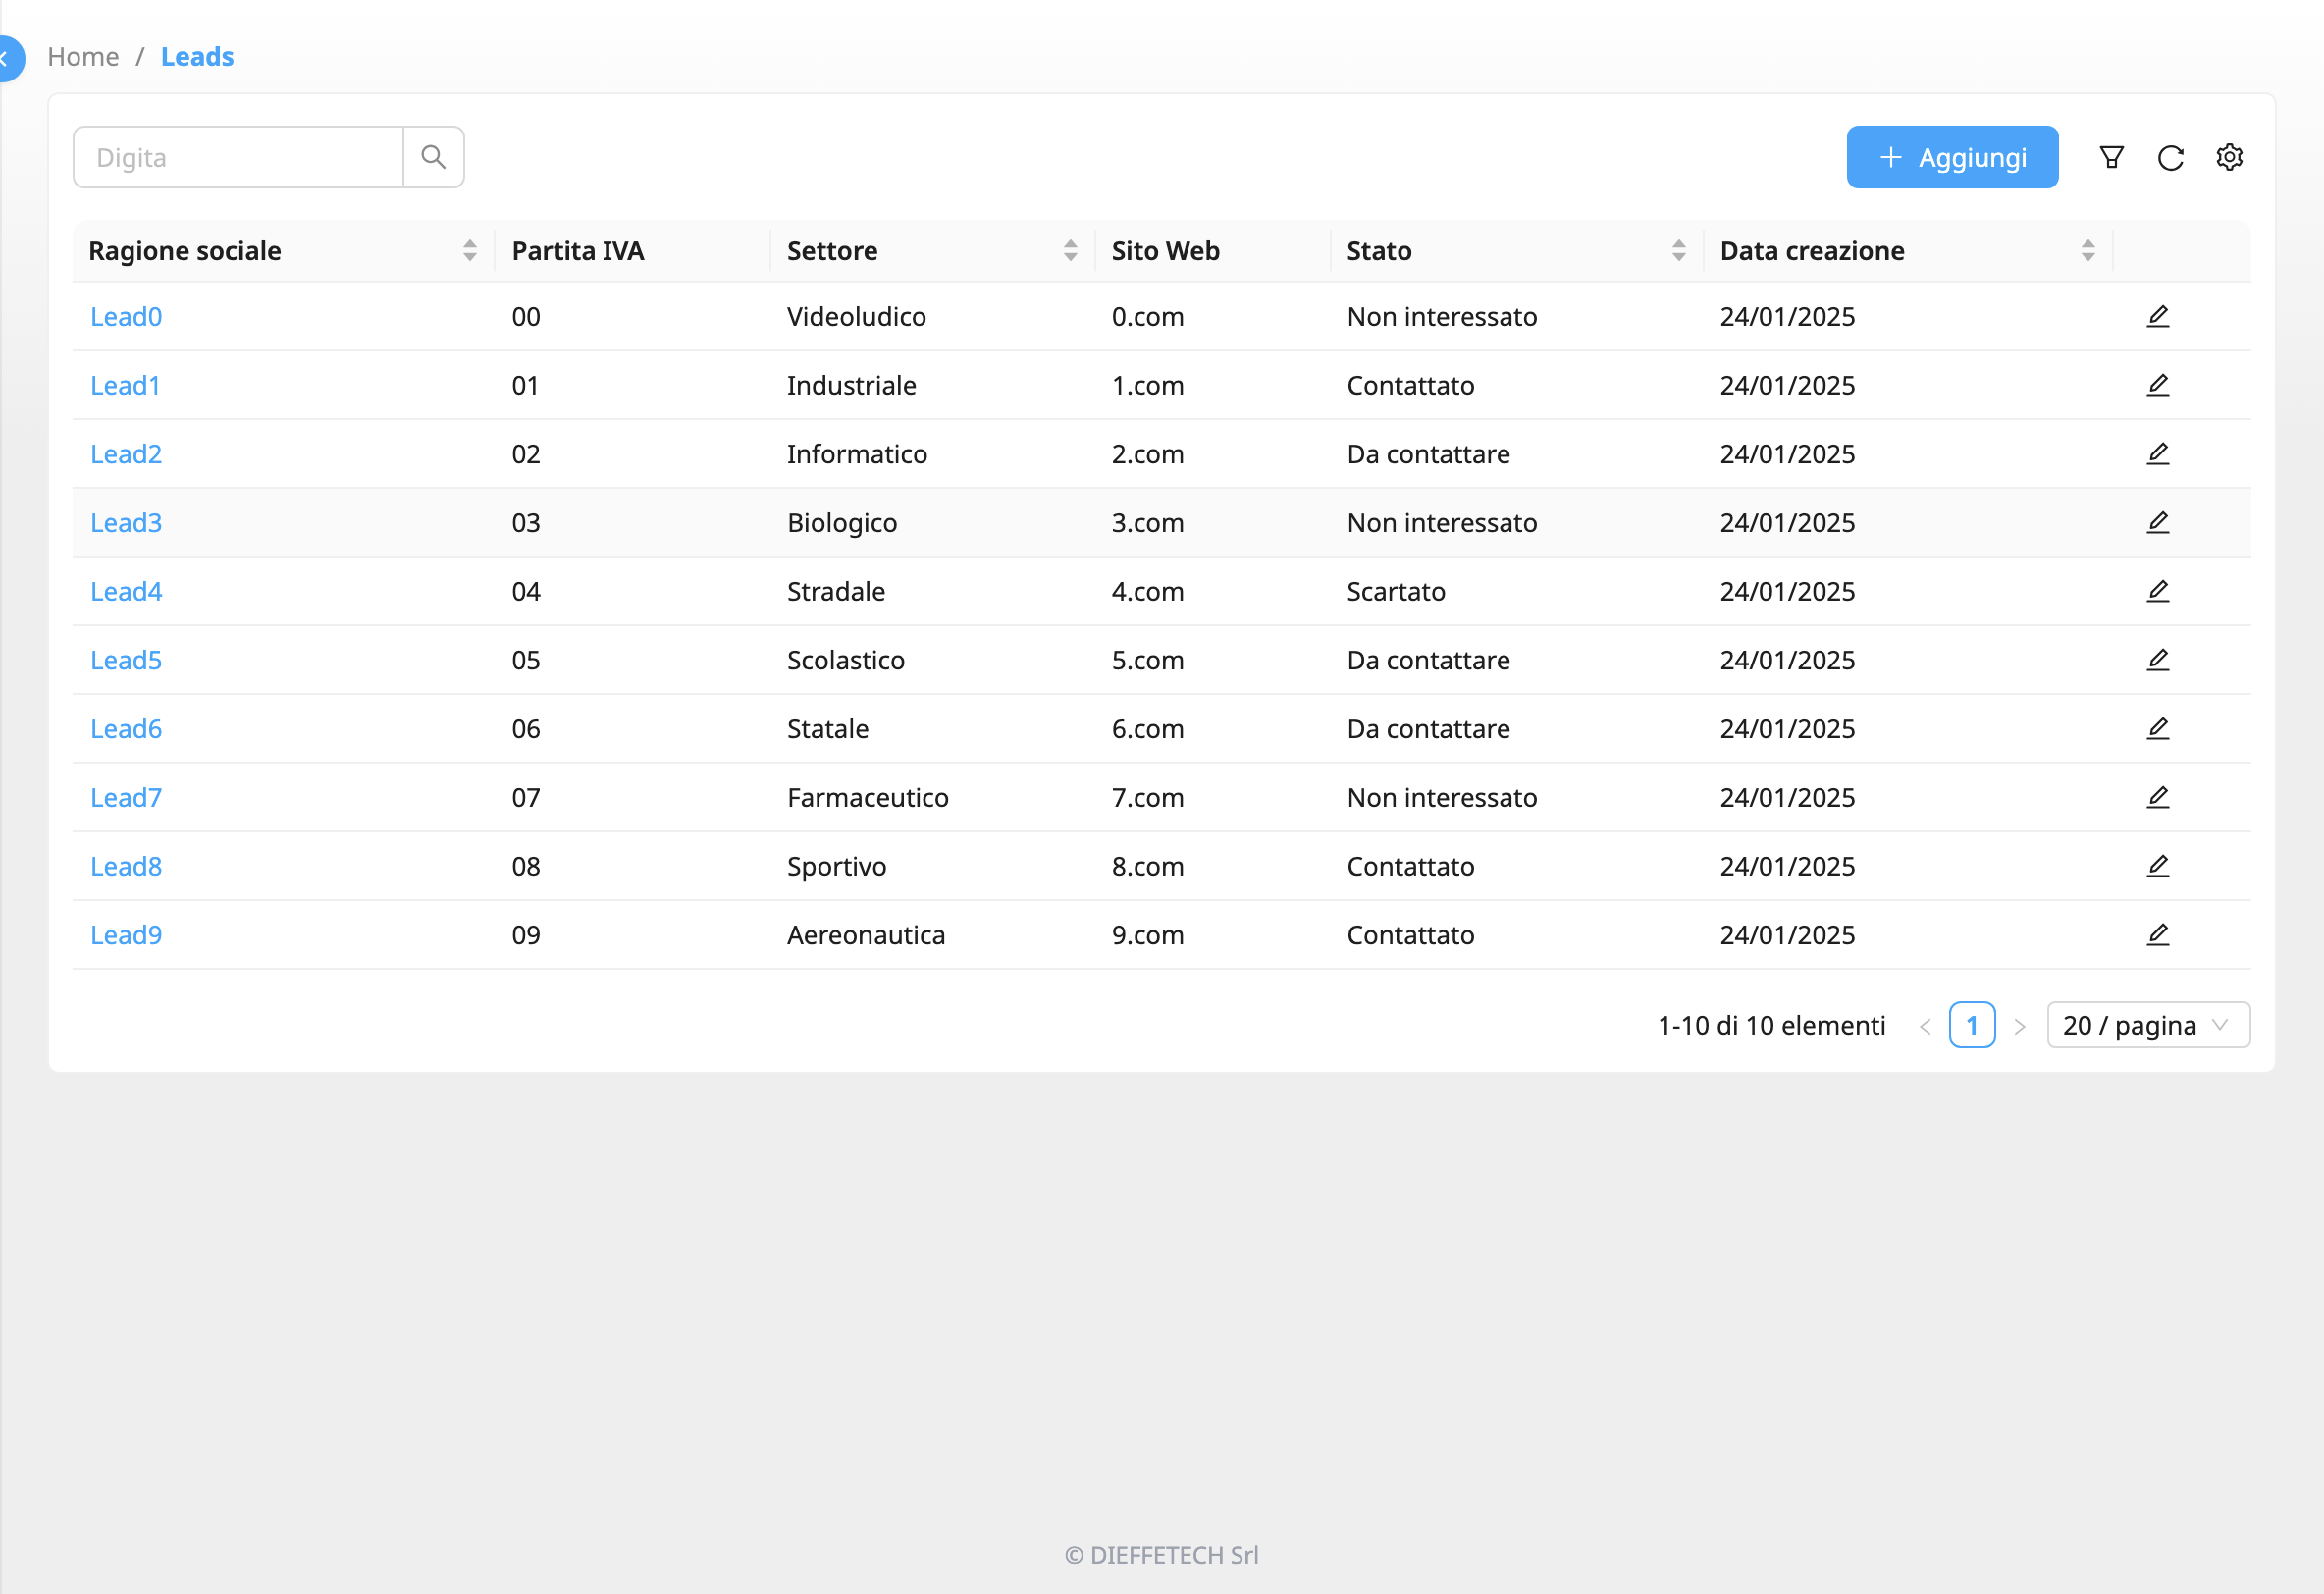
\includegraphics[width=1.0\textwidth]{immagini/LeadsTable.png}
	\caption{Tabella dei Leads.}
	\label{fig:leads_table}
\end{figure}
Nella figura \ref{fig:leads_table} è possibile osservare una visualizzazione che mostra esclusivamente i Leads. Ciò avviene grazie al valore della colonna \texttt{is\_customer} passato come parametro alle props di \texttt{CrudDataTable}. In particolare, questo parametro viene gestito all'interno della proprietà \texttt{params}. Quando si visualizza la tabella dei Clienti, \texttt{is\_customer} è impostato a \texttt{true}, mentre nella tabella dei Leads è impostato a \texttt{false}.

\subsection{Configurazione della CrudDataTable}
Il codice relativo alla \texttt{CrudDataTable}, presenta numerose proprietà che regolano il comportamento e la struttura della tabella:

\begin{itemize}
    \item \textbf{url}: esegue la chiamata fetch al database per ottenere i dati da visualizzare.
    \item \textbf{form}: definisce il form di creazione, che viene visualizzato al click sul pulsante \texttt{+Aggiungi}.
    \item \textbf{params}: Sono i parametri che vengono passati in backend, aggiunti come filtri di ricerca.
    \item \textbf{columns}: specifica l'elenco delle colonne da visualizzare nella tabella, con:
    \begin{itemize}
        \item \texttt{title}: il nome della colonna.
        \item \texttt{dataIndex}: il campo della tabella su cui si basa la colonna.
        \item \texttt{detail/sorter/search}: attributi booleani che definiscono se la colonna può essere filtrata, ordinata o ricercata.
    \end{itemize}
    \item \textbf{tabs}: Gestisce le sezioni di dettaglio visualizzabili al click su un elemento della tabella. Le tabs contengono \texttt{items}, ciascuno con:
    \begin{itemize}
        \item \texttt{label}: il nome della sezione.
        \item \texttt{key}: l'identificativo univoco della tab.
        \item \texttt{children}: il contenuto visualizzato all'interno della tab (a sua volta una CrudDataTable).
    \end{itemize}
\end{itemize}
\begin{lstlisting}[language=JavaScript, caption=Customers Table Code, label=customers_table_code, numbers=none]
export const CustomersTable = () => {
    const { t } = useTranslation();
    
    return (
        <CrudDataTable
          url={"/customers"}
          form={CustomerForm}
          params={{
            is_customer: true,
          }}
          tabs={(item) => {
            return [
              {
                label: t("Referenti"),
                key: "referents",
                children: (
                  <ReferentTable url={`/customers/${item?.id}/referents`} />
                ),
              },
              {
                label: t("Appuntamenti"),
                key: "appointments",
                children: (
                  <AppointmentsTable url={`/customers/${item?.id}/appointments`} />
                ),
              },
              {
                label: t("Task"),
                key: "customer-tasks",
                children: (
                  <CustomerTasksTable url={`/customers/${item?.id}/customer-tasks`} />
                ),
              },
              {
                label: t("Offerte"),
                key: "offers",
                children: (
                  <CustomerOffersTable url={`/customers/${item?.id}/offers`} />
                ),
              },
            ];
          }}
          columns={[
            {
              title: t("Ragione sociale"),
              dataIndex: "business_name",
              detail: true,
              sorter: true,
              search: true,
            },
            ...
          ]}
        />
      );
    };
    \end{lstlisting}
    Una visione più dettagliata del comportamento delle tabs può essere osservata nel codice riportato in \ref{customers_table_code}. Quando si clicca sul dettaglio di un Cliente o Lead, vengono visualizzate diverse sezioni: \textit{Referenti}, \textit{Appuntamenti}, \textit{Task} e \textit{Offerte}. Ognuna di queste sezioni è rappresentata da una tabella dedicata, che viene popolata tramite una chiamata API, la quale restituisce i dati specifici del Cliente o Lead selezionato.
    
    La chiamata API utilizza il seguente formato per i parametri:\\
    \texttt{/customers/item?.id/key}, dove \texttt{item?.id} rappresenta l'ID univoco del Cliente o Lead attualmente selezionato, e \texttt{key} identifica la sezione richiesta (ad esempio, \textit{referents}, \textit{appointments}, \textit{tasks} o \textit{offers}).
    
    Nel caso specifico della colonna "Ragione Sociale", notiamo che il parametro \texttt{detail} è impostato su \texttt{true}. Questo significa che il nome visualizzato nella colonna viene reso interattivo (come si può osservare nella tabella in Figura \ref{fig:leads_table}, dove i nomi sono evidenziati in azzurro). Cliccando su uno di questi nomi, si apre la schermata dei dettagli del Cliente o Lead (\ref{fig:leads_details}), in cui è possibile accedere e navigare tra le varie sezioni di dettaglio.\begin{figure}[H]
	\centering
	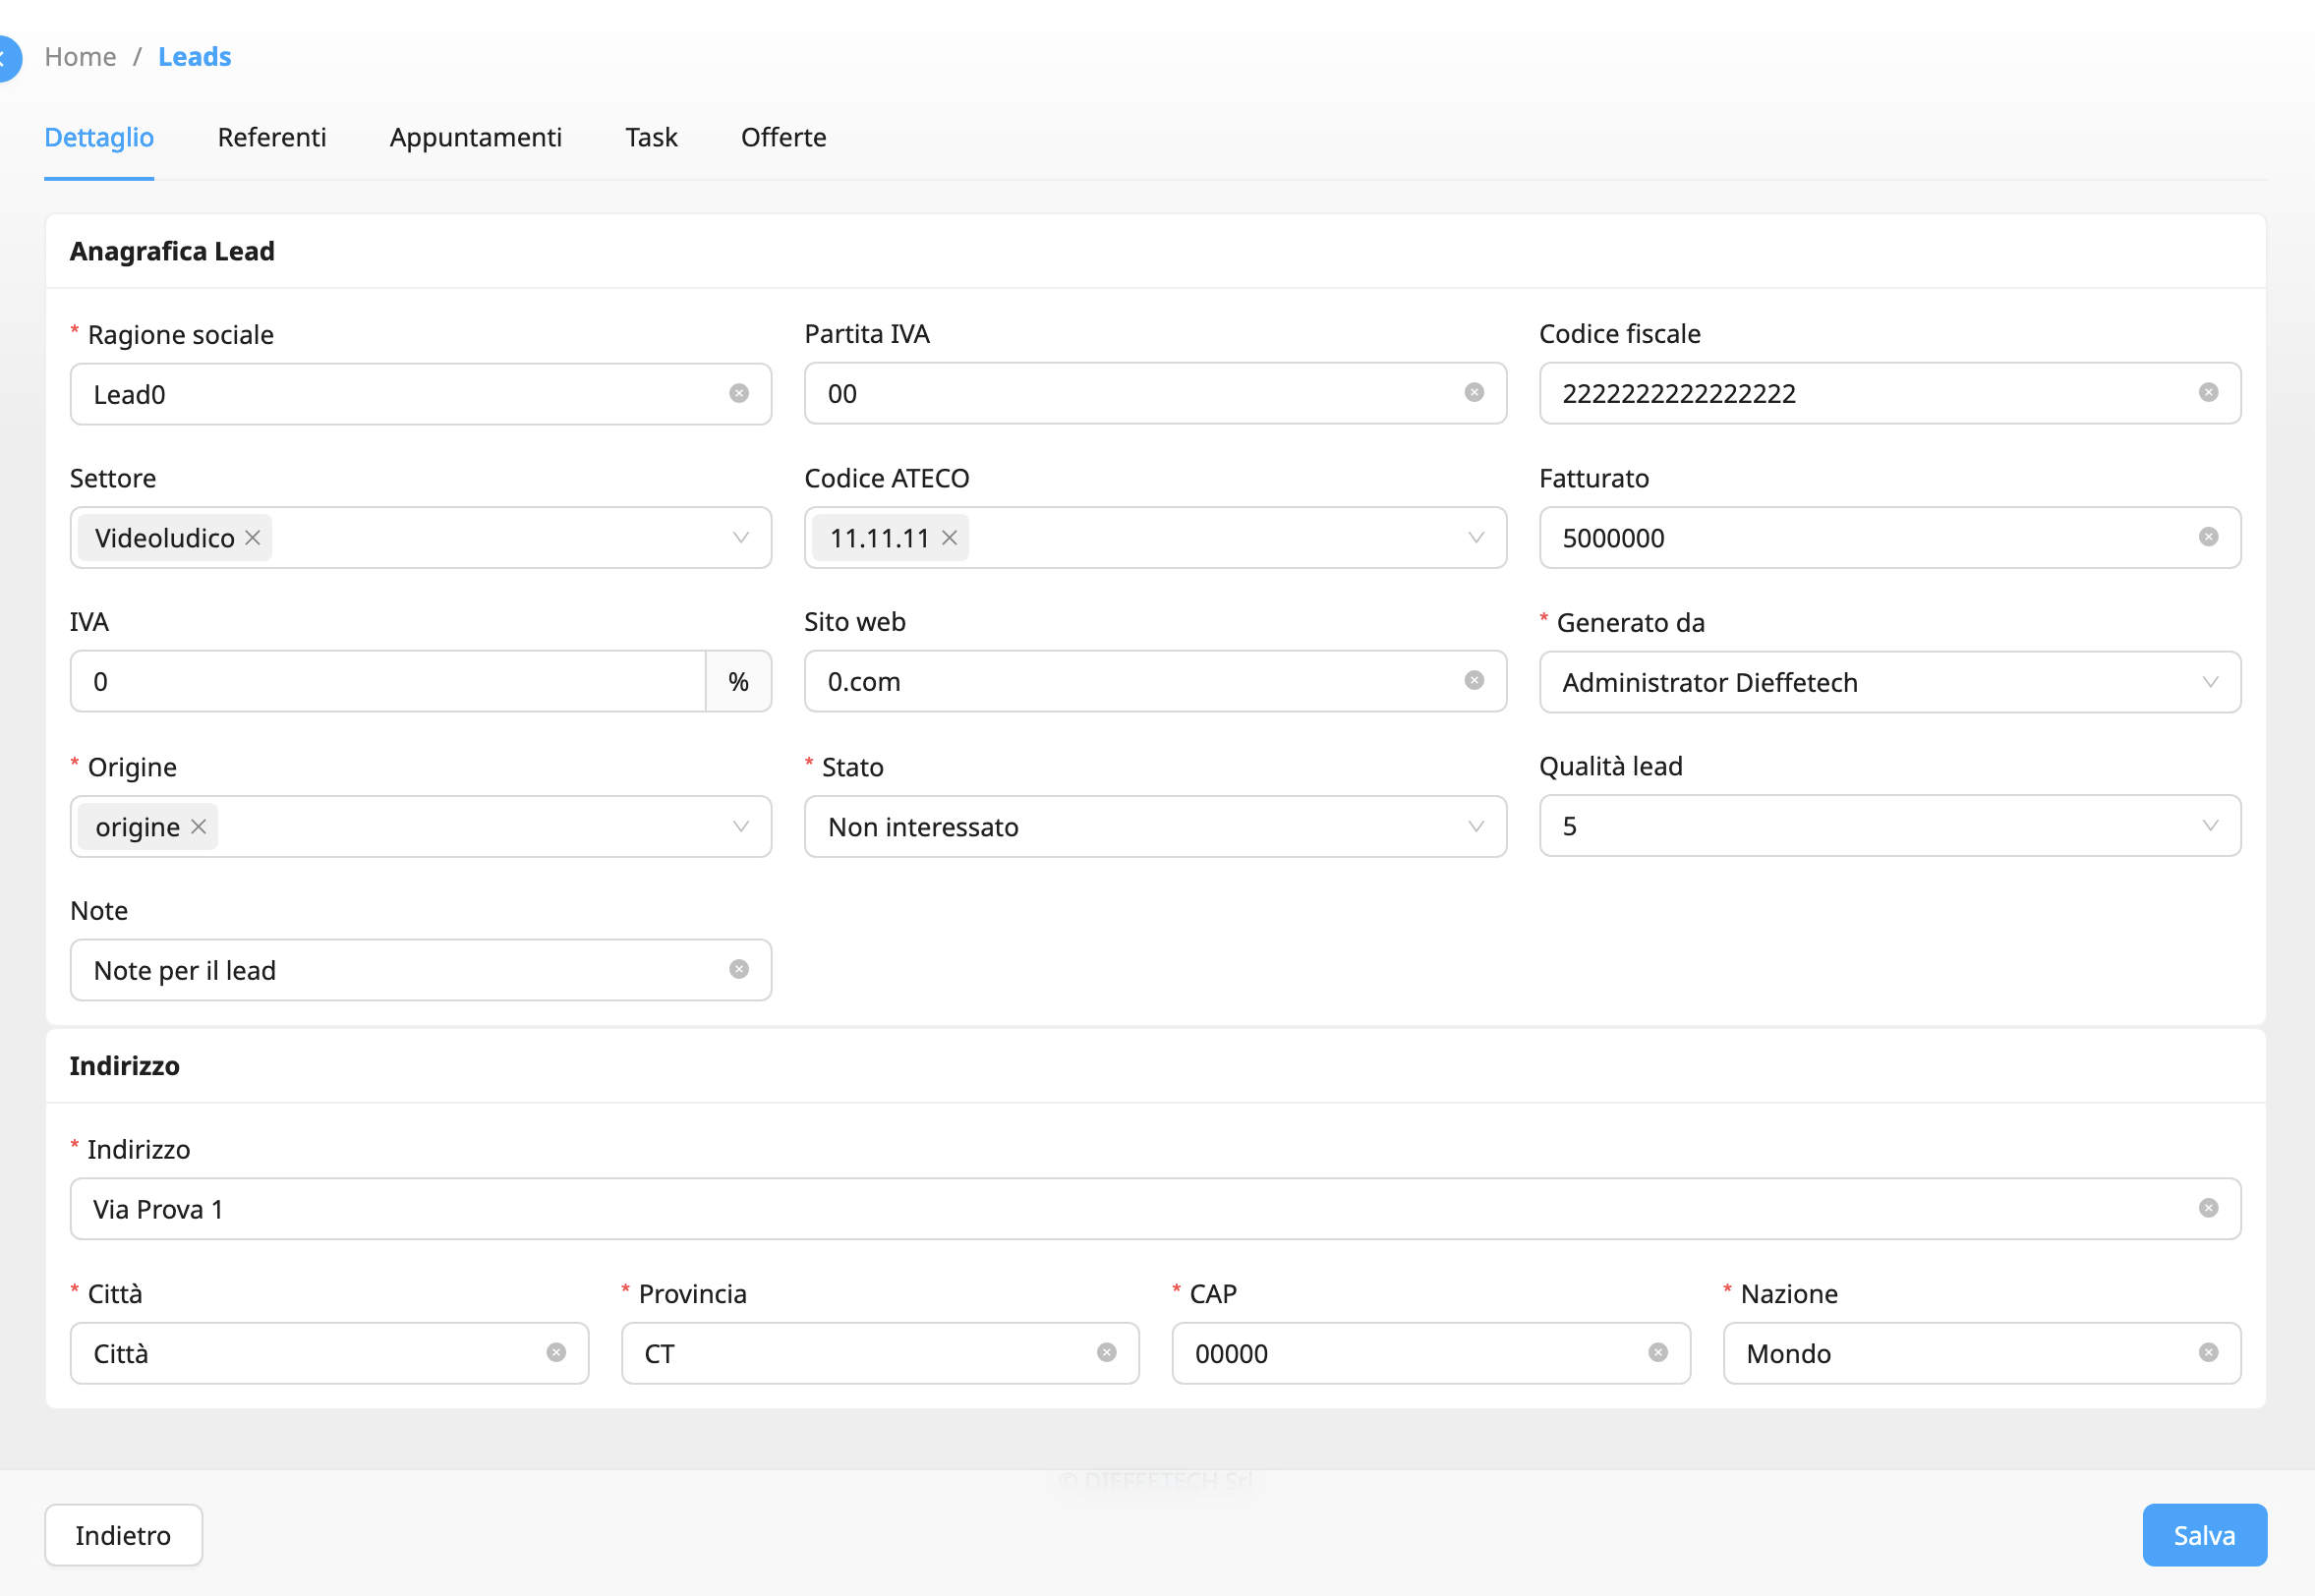
\includegraphics[width=1.0\textwidth]{immagini/LeadsDetails.png}
	\caption{Dettagli di un Lead.}
	\label{fig:leads_details}
\end{figure}

\section{Appuntamenti}\label{sec:cap_sec_subsec_appuntamenti}
In questa sezione vengono gestiti gli appuntamenti, visualizzati e organizzati all'interno di una tabella specifica, che può essere vista nella Figura \ref{fig:appointments_table}. La tabella è parte della componente \texttt{CrudDataTable}, la quale consente la gestione dinamica dei dati. Ogni colonna della tabella è definita da proprietà come \texttt{title}, \texttt{dataIndex}, e altre opzioni che permettono di abilitare il filtraggio o l'ordinamento.

La tabella degli appuntamenti ha collegamenti con altre entità del sistema, tra cui la tabella dei referenti (che permette di selezionare un referente specifico per ogni appuntamento, associato al cliente selezionato) e la tabella degli utenti (che permette di associare un utente registrato nel sistema, all'appuntamento). Questi collegamenti vengono gestiti attraverso le relazioni \texttt{Eloquent} definite nel Model di \texttt{Appointments}. Queste relazioni permettono di navigare facilmente tra i dati correlati e semplificano la gestione delle associazioni all'interno del database.

\begin{figure}[ht]
	\centering
	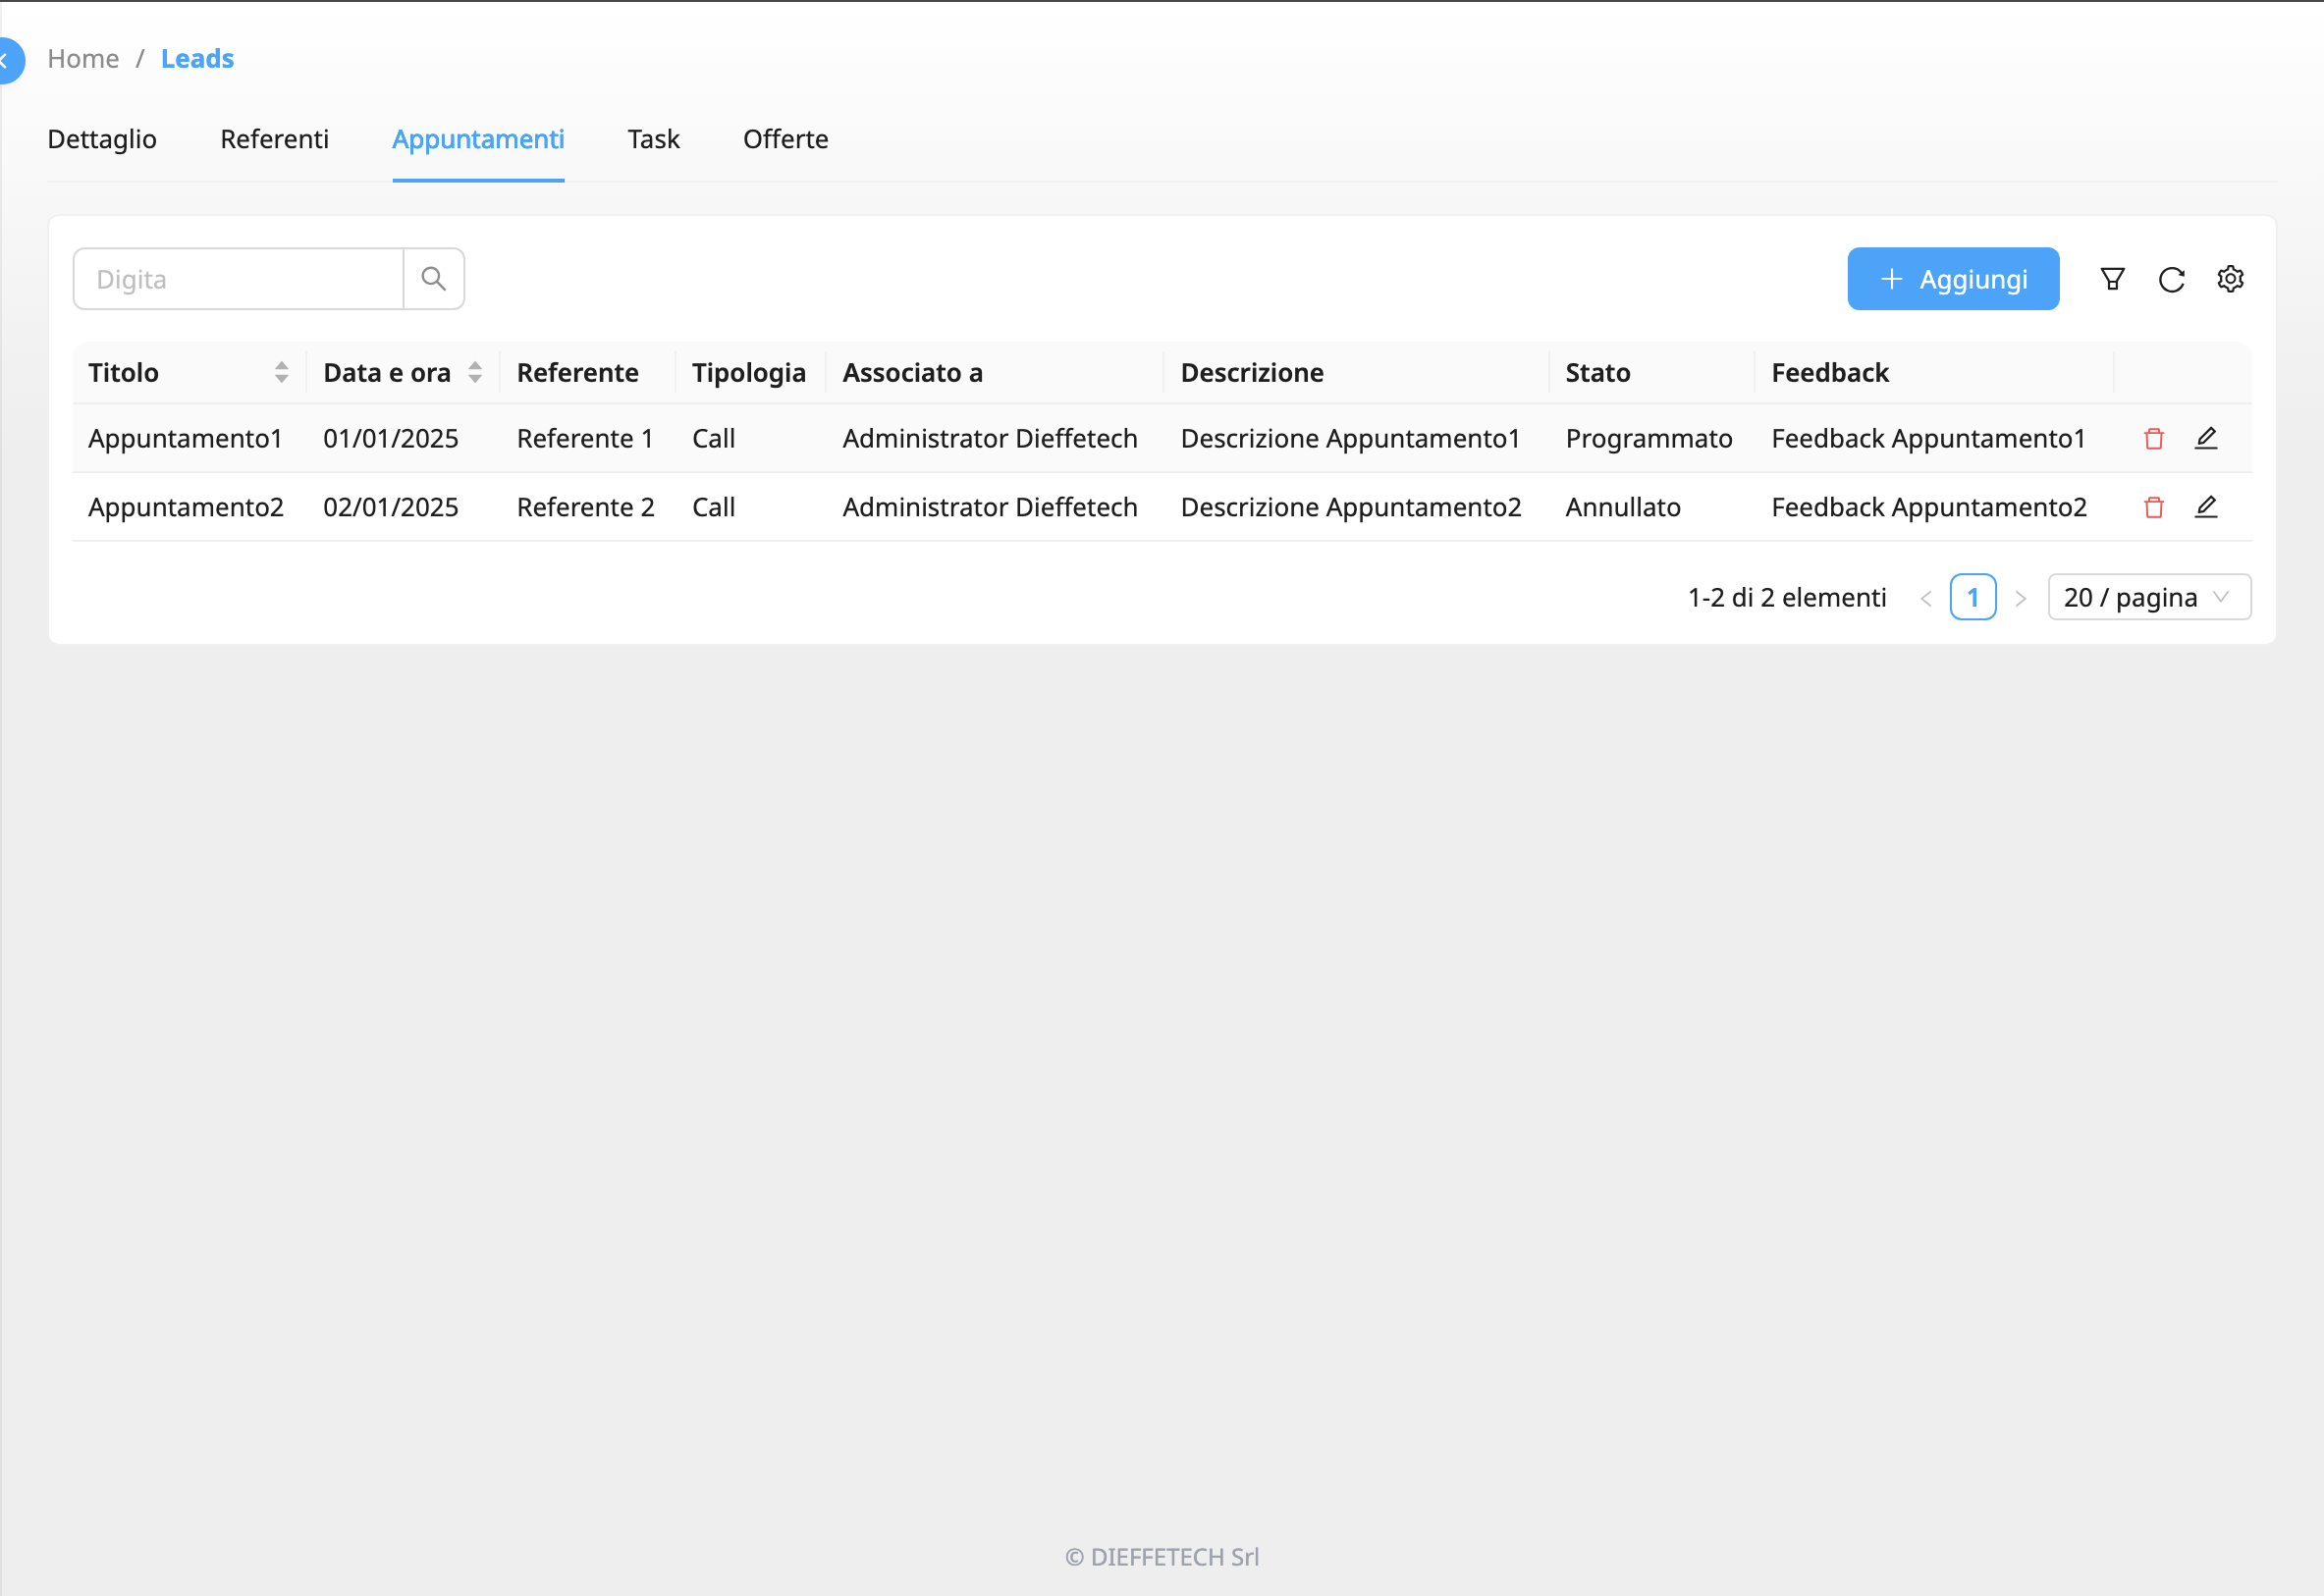
\includegraphics[width=1.0\textwidth]{immagini/AppointmentsTable.png}
	\caption{Tabella degli appuntamenti.}
	\label{fig:appointments_table}
\end{figure}

Oltre alla tabella, la gestione degli appuntamenti include anche la possibilità di creare nuovi appuntamenti attraverso un form dedicato, visualizzato nella Figura \ref{fig:appointments_form}. Questo form consente di compilare i campi necessari per l'inserimento di un nuovo appuntamento, tra cui il nome del referente e l'utente associato. Ogni campo del form è definito all'interno del componente \texttt{AppointmentsForm}, che si occupa di validare i dati inseriti dall'utente e inviarli al backend per il salvataggio nel database. Anche qui, i campi collegati con altre entità, come i referenti e gli utenti, vengono popolati dinamicamente grazie alle relazioni \texttt{Eloquent}.
\begin{figure}[ht]
	\centering
	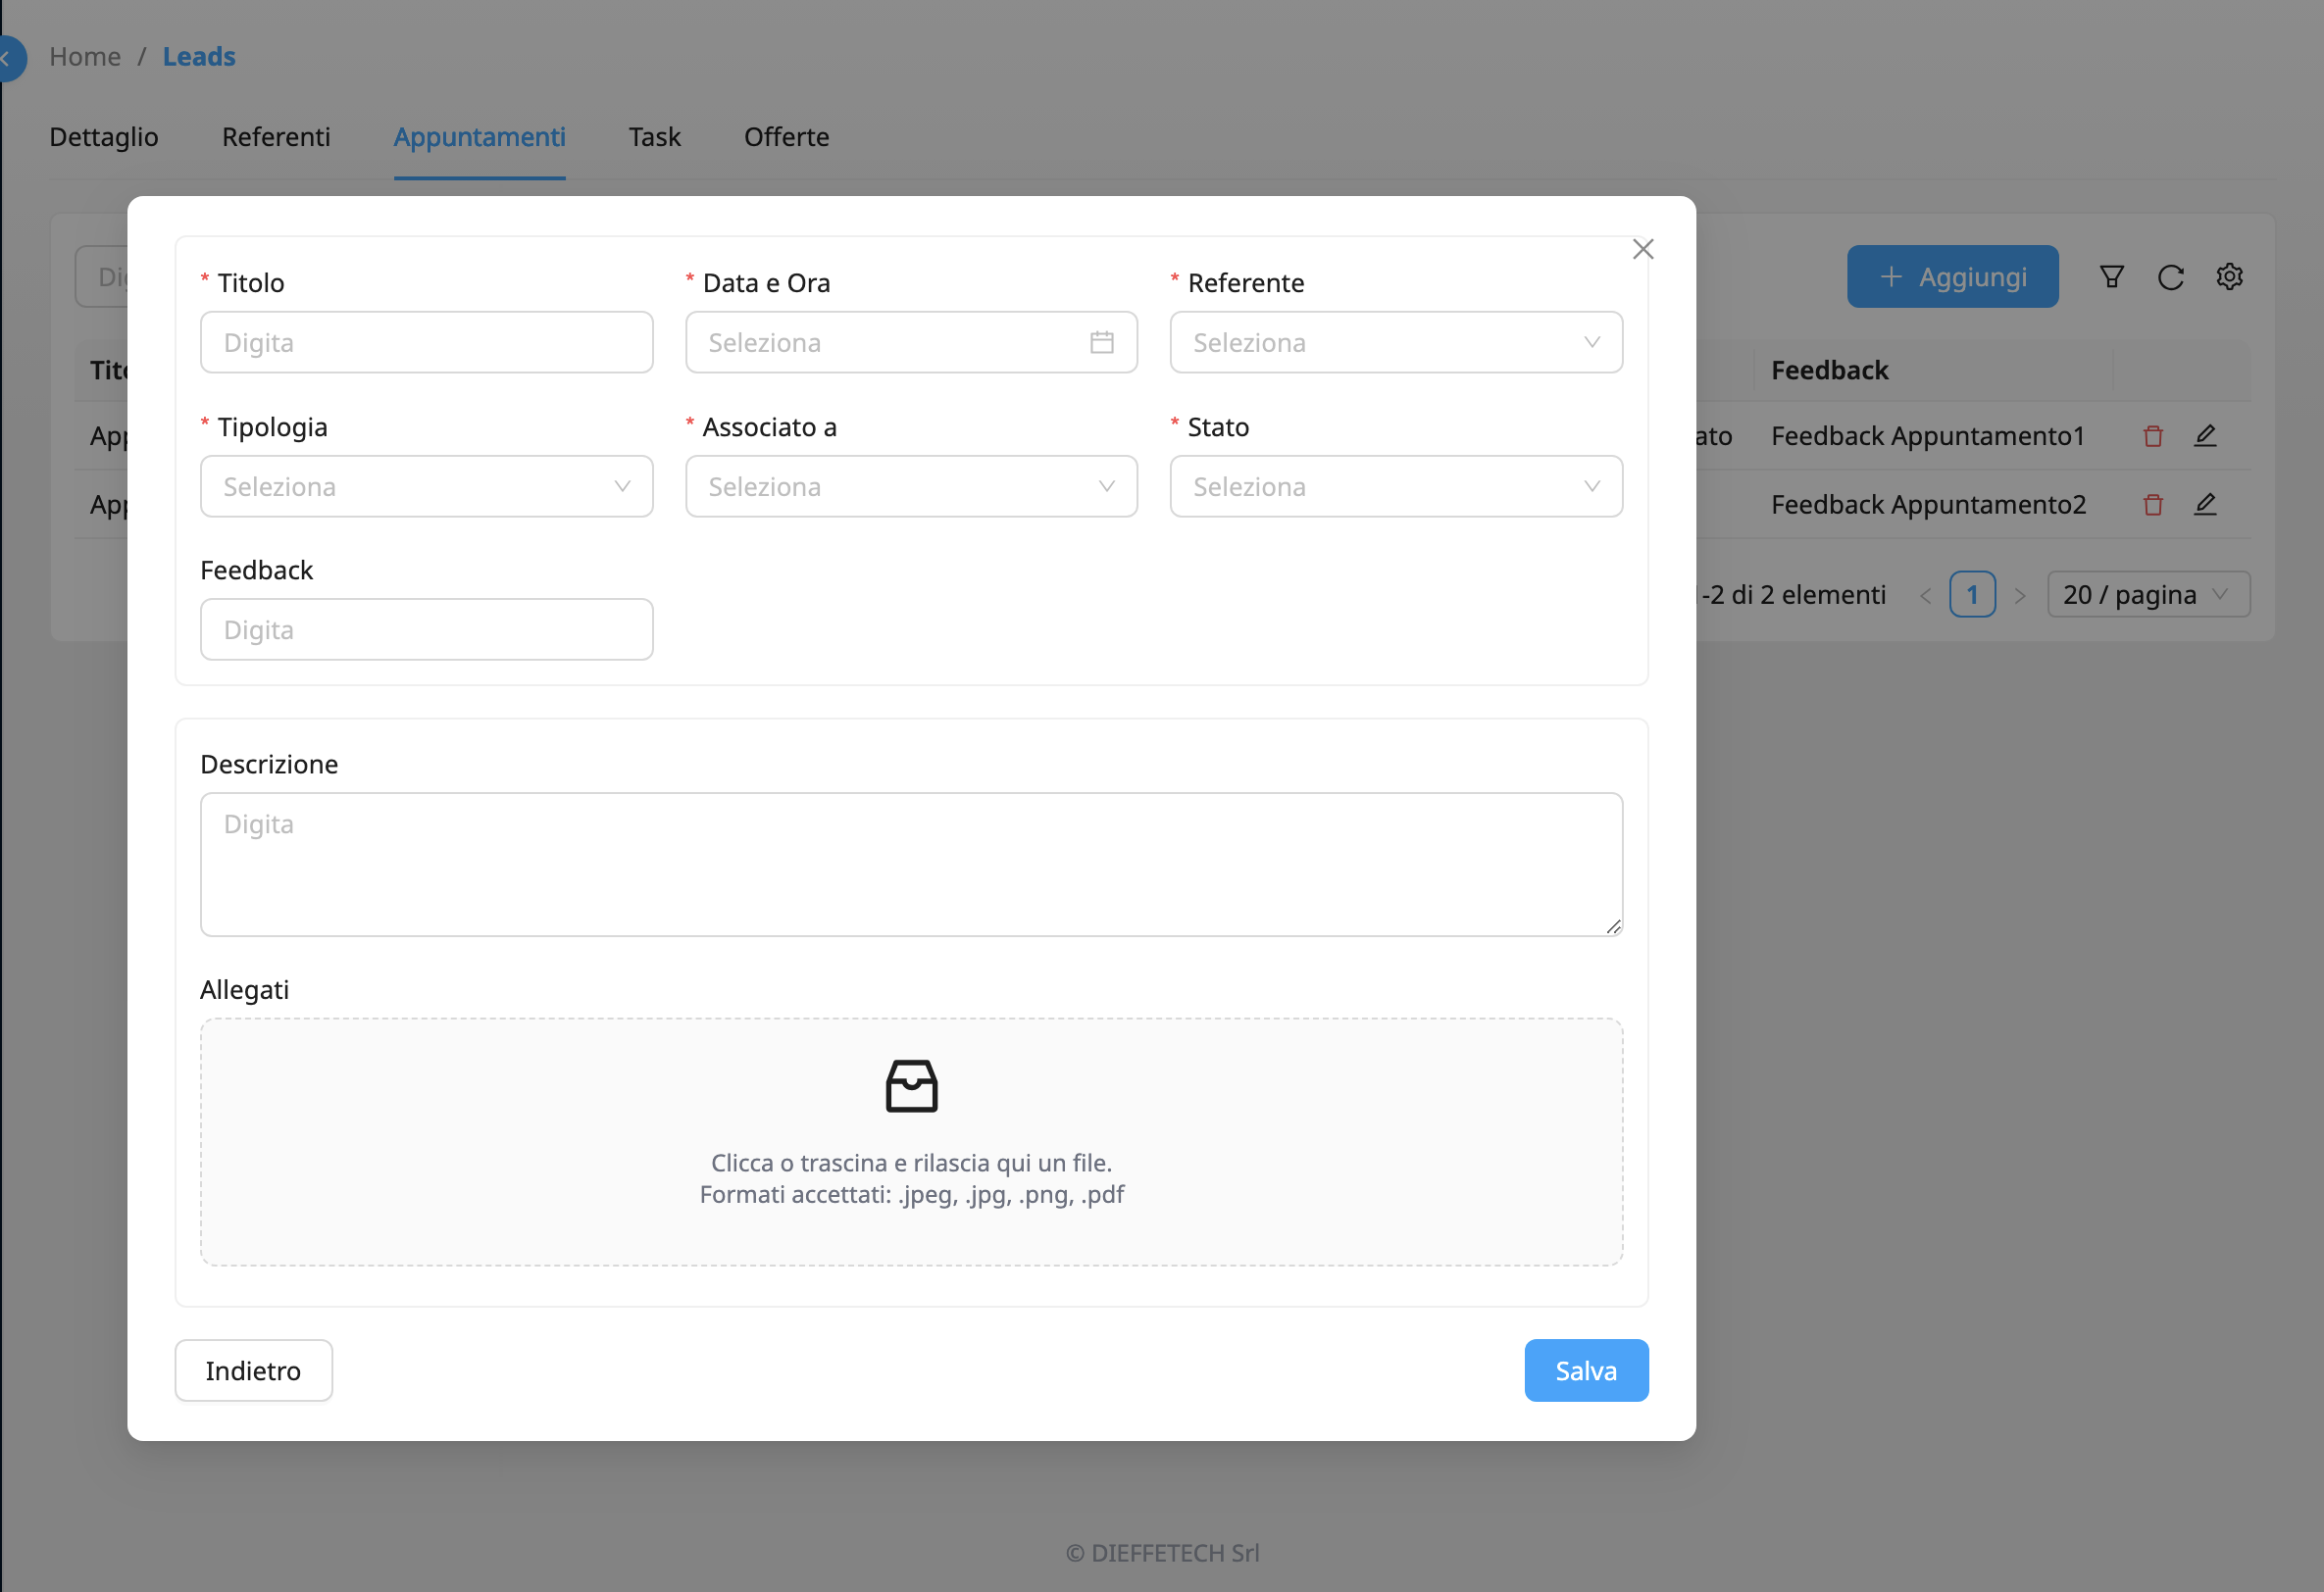
\includegraphics[width=1.0\textwidth]{immagini/AppointmentsForm.png}
	\caption{Form degli appuntamenti.}
	\label{fig:appointments_form}
\end{figure}

Entrando nel Model degli Appuntamenti, infatti, possiamo osservare che nella sezione dedicata alle funzioni di relazione troviamo il seguente codice:
\begin{lstlisting}[language=JavaScript, numbers=none]
public function customer(): BelongsTo
{
    return $this->belongsTo(related: Customer::class);
}
public function referent(): BelongsTo
{
    return $this->belongsTo(related: Referent::class);
}
public function userAdmin(): BelongsTo
{
    return $this->belongsTo(related: UserAdmin::class);
}    
\end{lstlisting}

\section{Task}\label{sec:cap_sec_subsec_task}
In questa sezione vengono gestiti i task, che sono simili agli appuntamenti nella loro organizzazione, ma presentano una differenza importante: ogni task è associato a un appuntamento specifico e ad un utente, mentre gli appuntamenti erano legati a un referente e a un utente.

I task sono visualizzati e organizzati all'interno di una tabella, come mostrato nella Figura \ref{fig:tasks_table}, utilizzando le stesse modalità degli appuntamenti, con la componente \texttt{CrudDataTable} e le relative proprietà per la gestione dinamica dei dati.

Un aspetto distintivo dei task è la relazione con la tabella degli appuntamenti, che consente di associare ogni task a un appuntamento specifico. Inoltre, come per gli appuntamenti, i task sono legati agli utenti, permettendo di assegnare un determinato compito a una persona all'interno dell'azienda. Queste relazioni vengono gestite tramite le definizioni \texttt{Eloquent} nel Model \texttt{Task}.

\begin{figure}[ht]
	\centering
	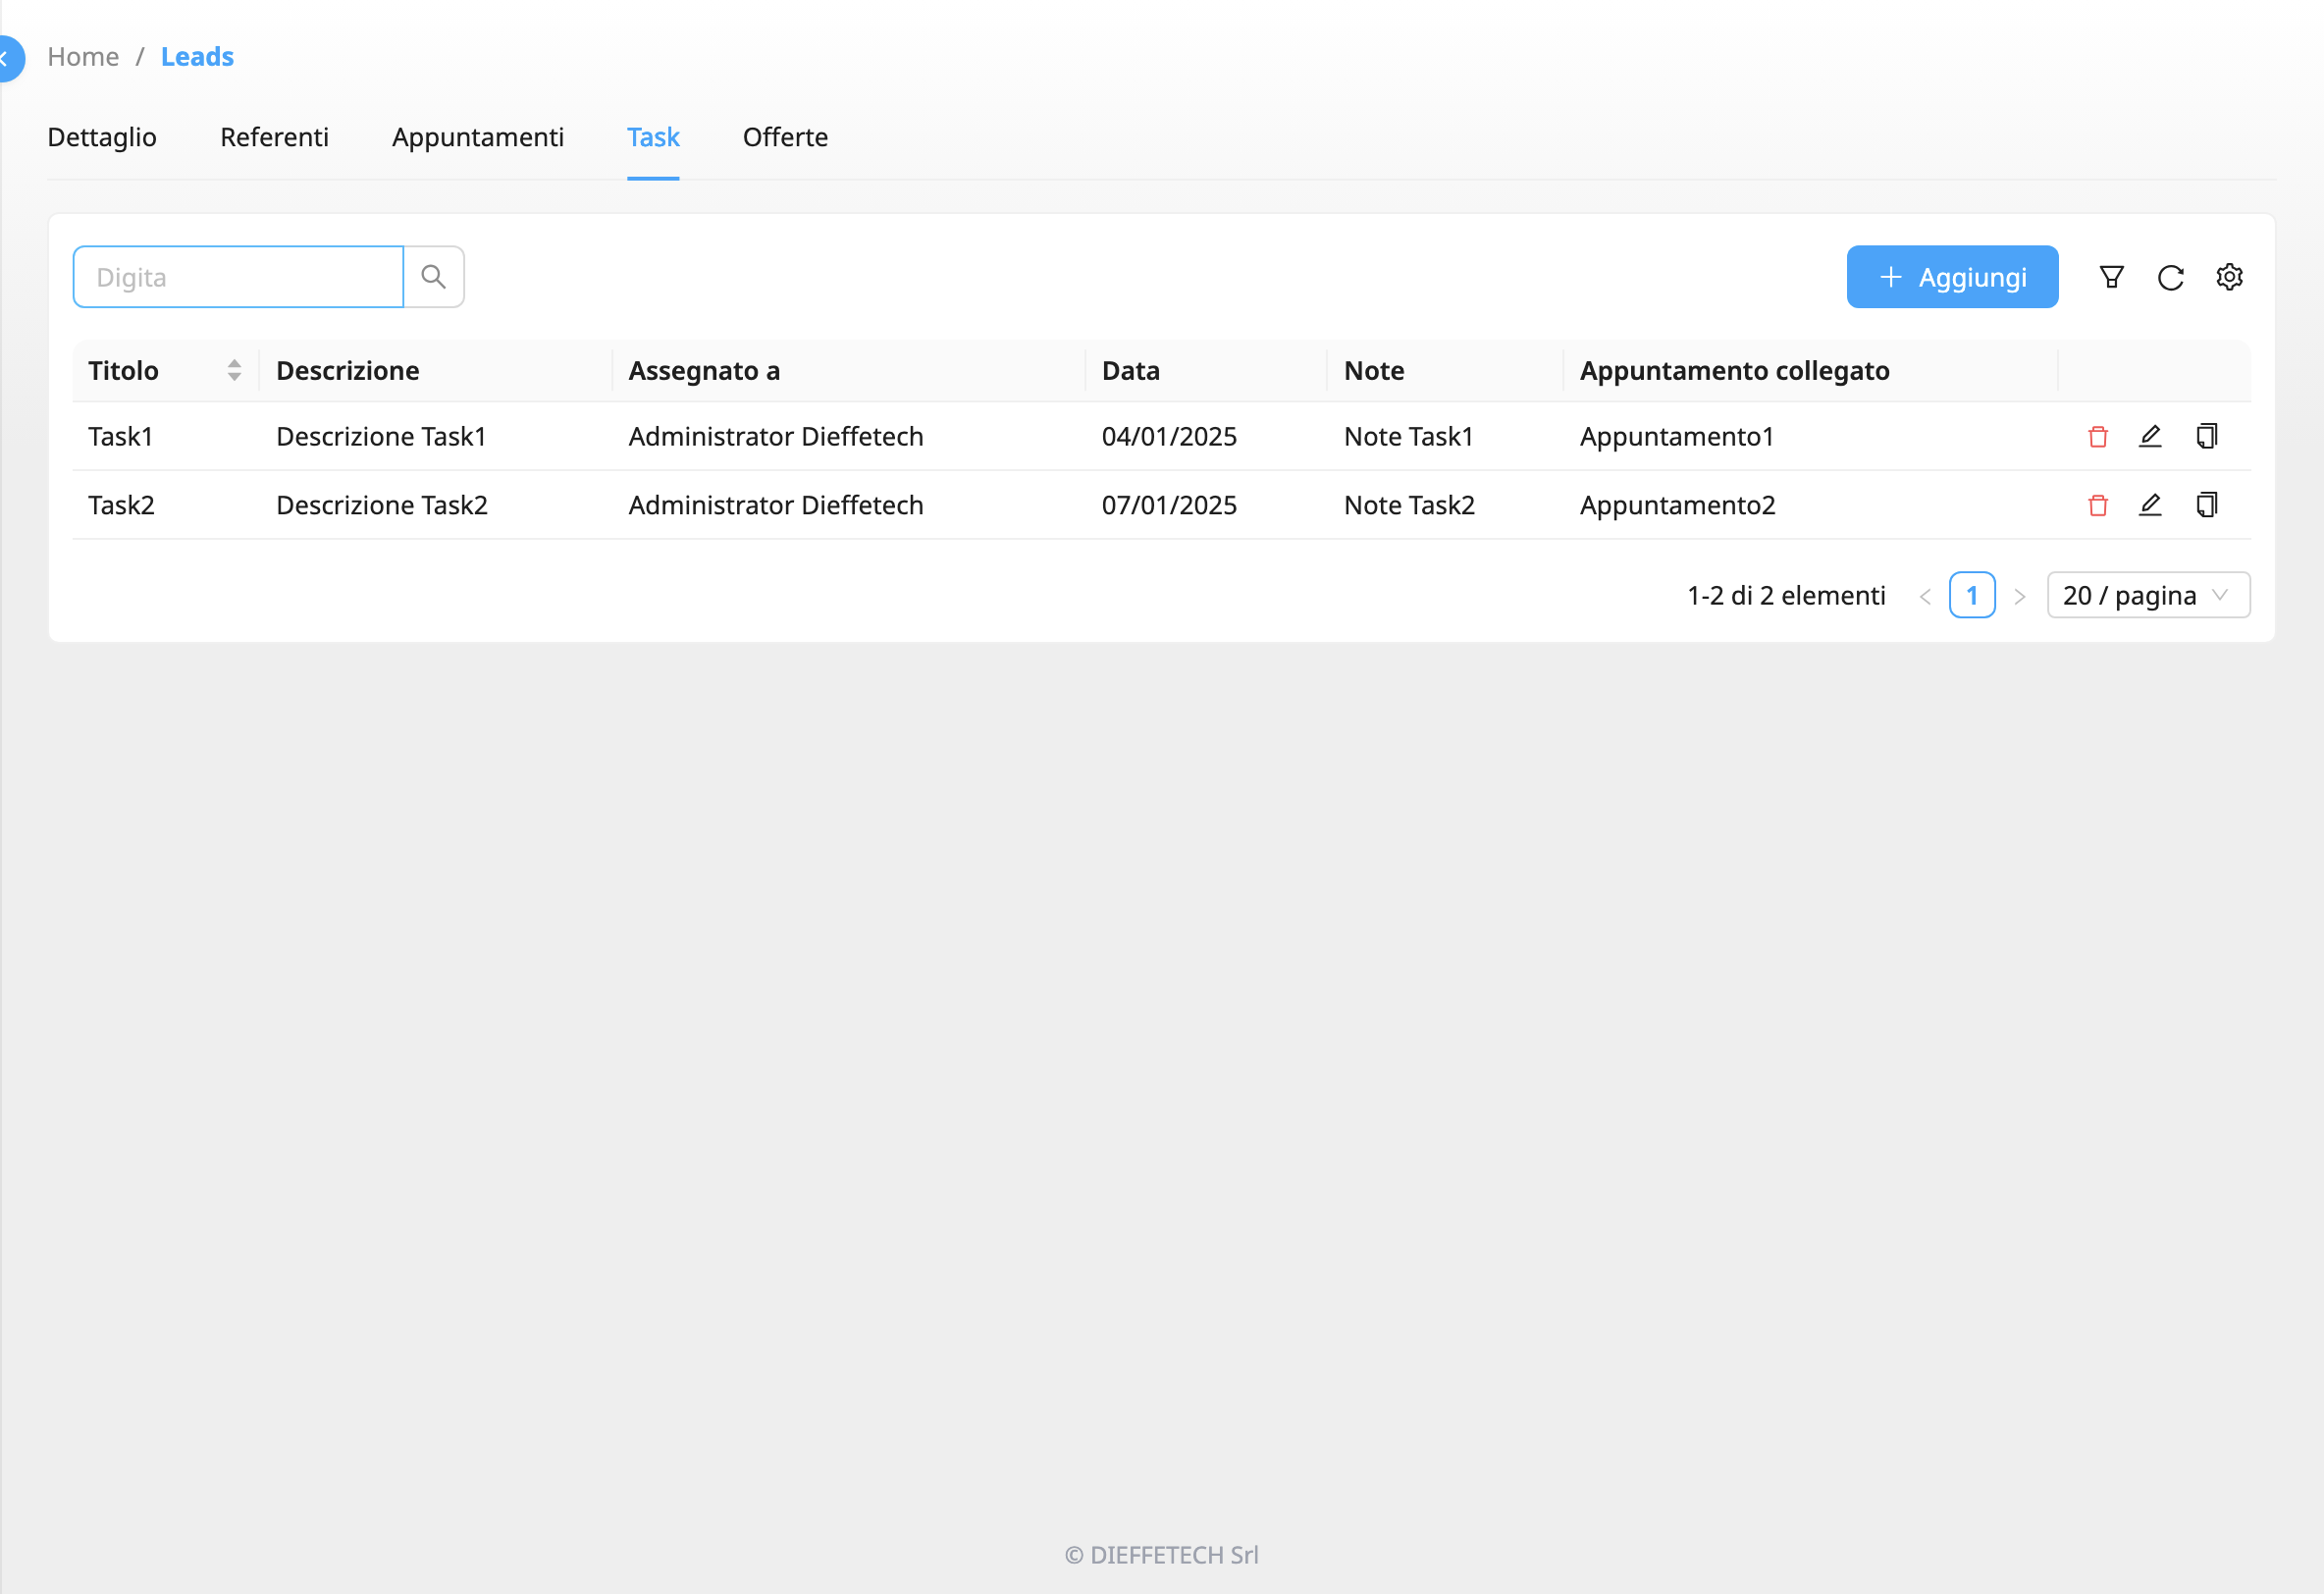
\includegraphics[width=1.0\textwidth]{immagini/TaskTable.png}
	\caption{Tabella dei task.}
	\label{fig:tasks_table}
\end{figure}

Oltre alla tabella, la gestione dei task include la possibilità di creare nuovi task tramite un form dedicato, mostrato nella Figura \ref{fig:tasks_form}. Il form consente di selezionare l'appuntamento associato e gli utenti coinvolti nel task. Ogni campo è definito nel componente \texttt{TaskForm}, che gestisce la validazione dei dati e l'invio al backend per il salvataggio nel database. Le relazioni tra i task, gli appuntamenti e gli utenti sono gestite dinamicamente grazie a \texttt{Eloquent}.

\begin{figure}[ht]
	\centering
	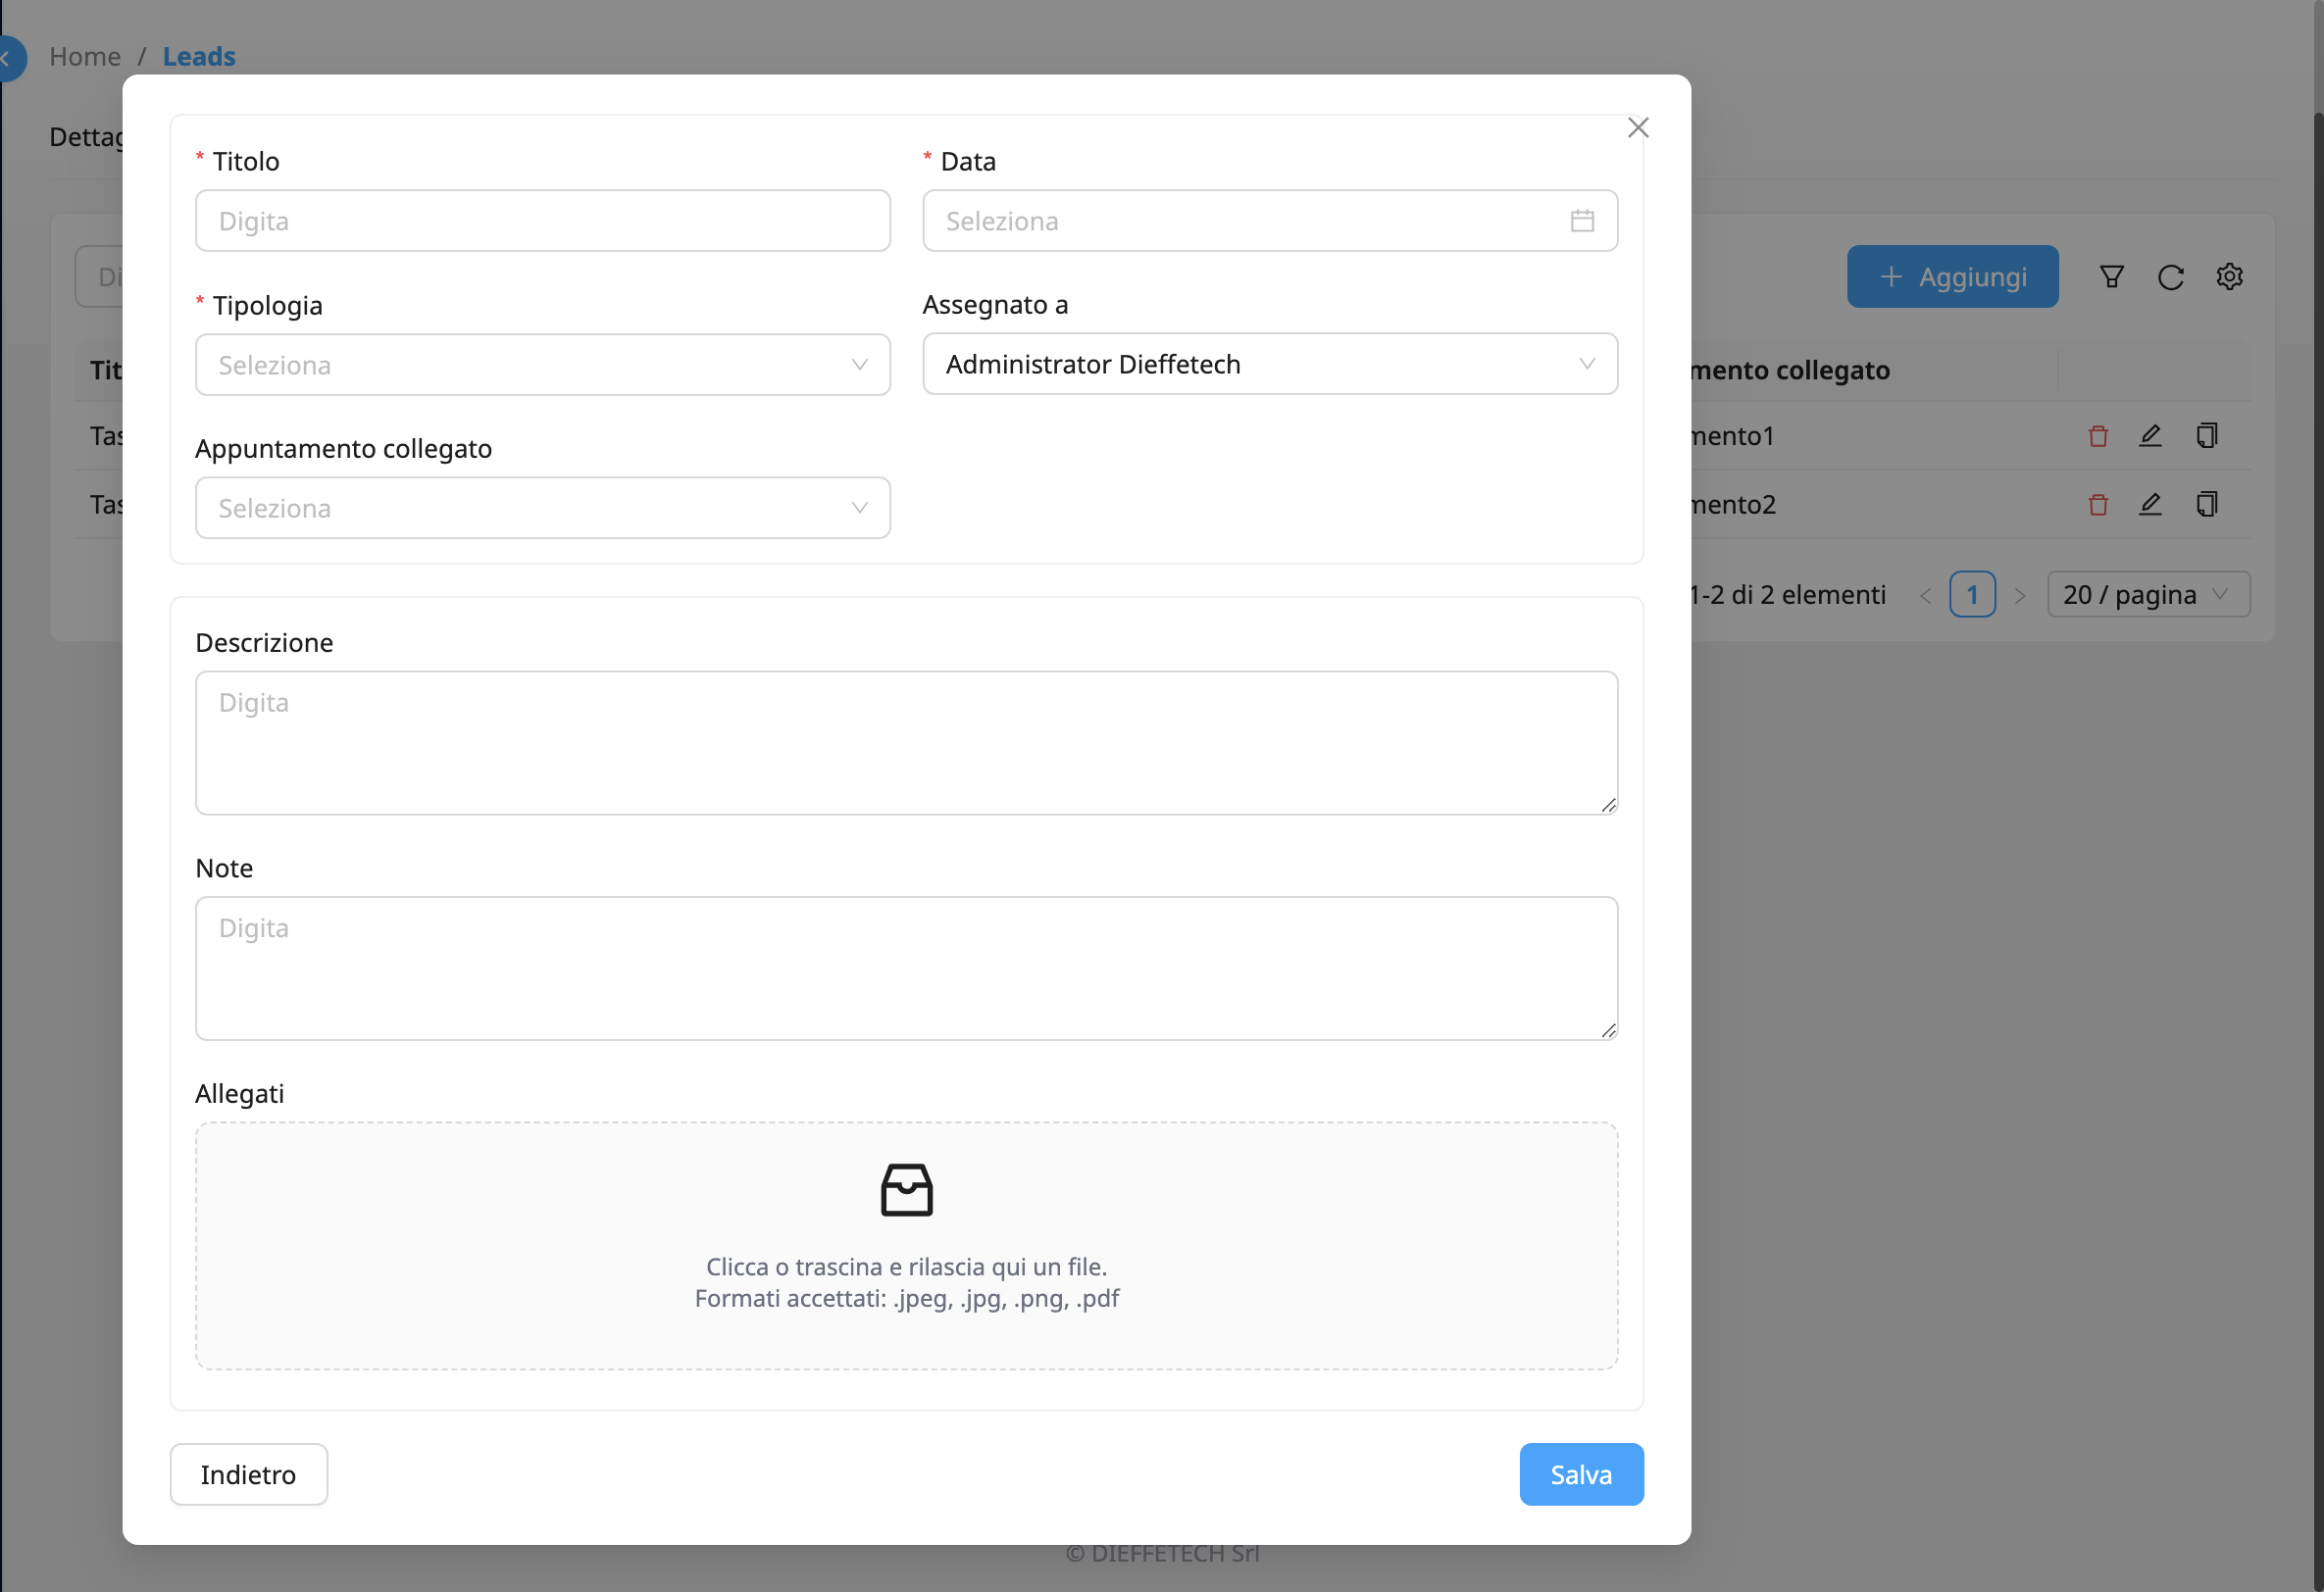
\includegraphics[width=1.0\textwidth]{immagini/TaskForm.png}
	\caption{Form dei task.}
	\label{fig:tasks_form}
\end{figure}
Nel Model dei Task, possiamo osservare che nella sezione dedicata alle funzioni di relazione troviamo il seguente codice:
\begin{lstlisting}[language=JavaScript, numbers=none]
public function customer(): BelongsTo
{
    return $this->belongsTo(related: Customer::class);
}    
public function appointment(): BelongsTo
{
    return $this->belongsTo(related: Appointment::class);
}
public function userAdmin(): BelongsTo
{
    return $this->belongsTo(related: UserAdmin::class);
}
\end{lstlisting}

\section{Offerte}\label{sec:cap_sec_subsec_offerte}
La sezione dedicata alle \textbf{offerte}  merita un’attenzione particolare, in quanto presenta una logica più complessa rispetto alle altre sezioni.  Inoltre, è l'unica ad avere una sezione dedicata nel baseMenu.

\begin{figure}[H]
    \centering
    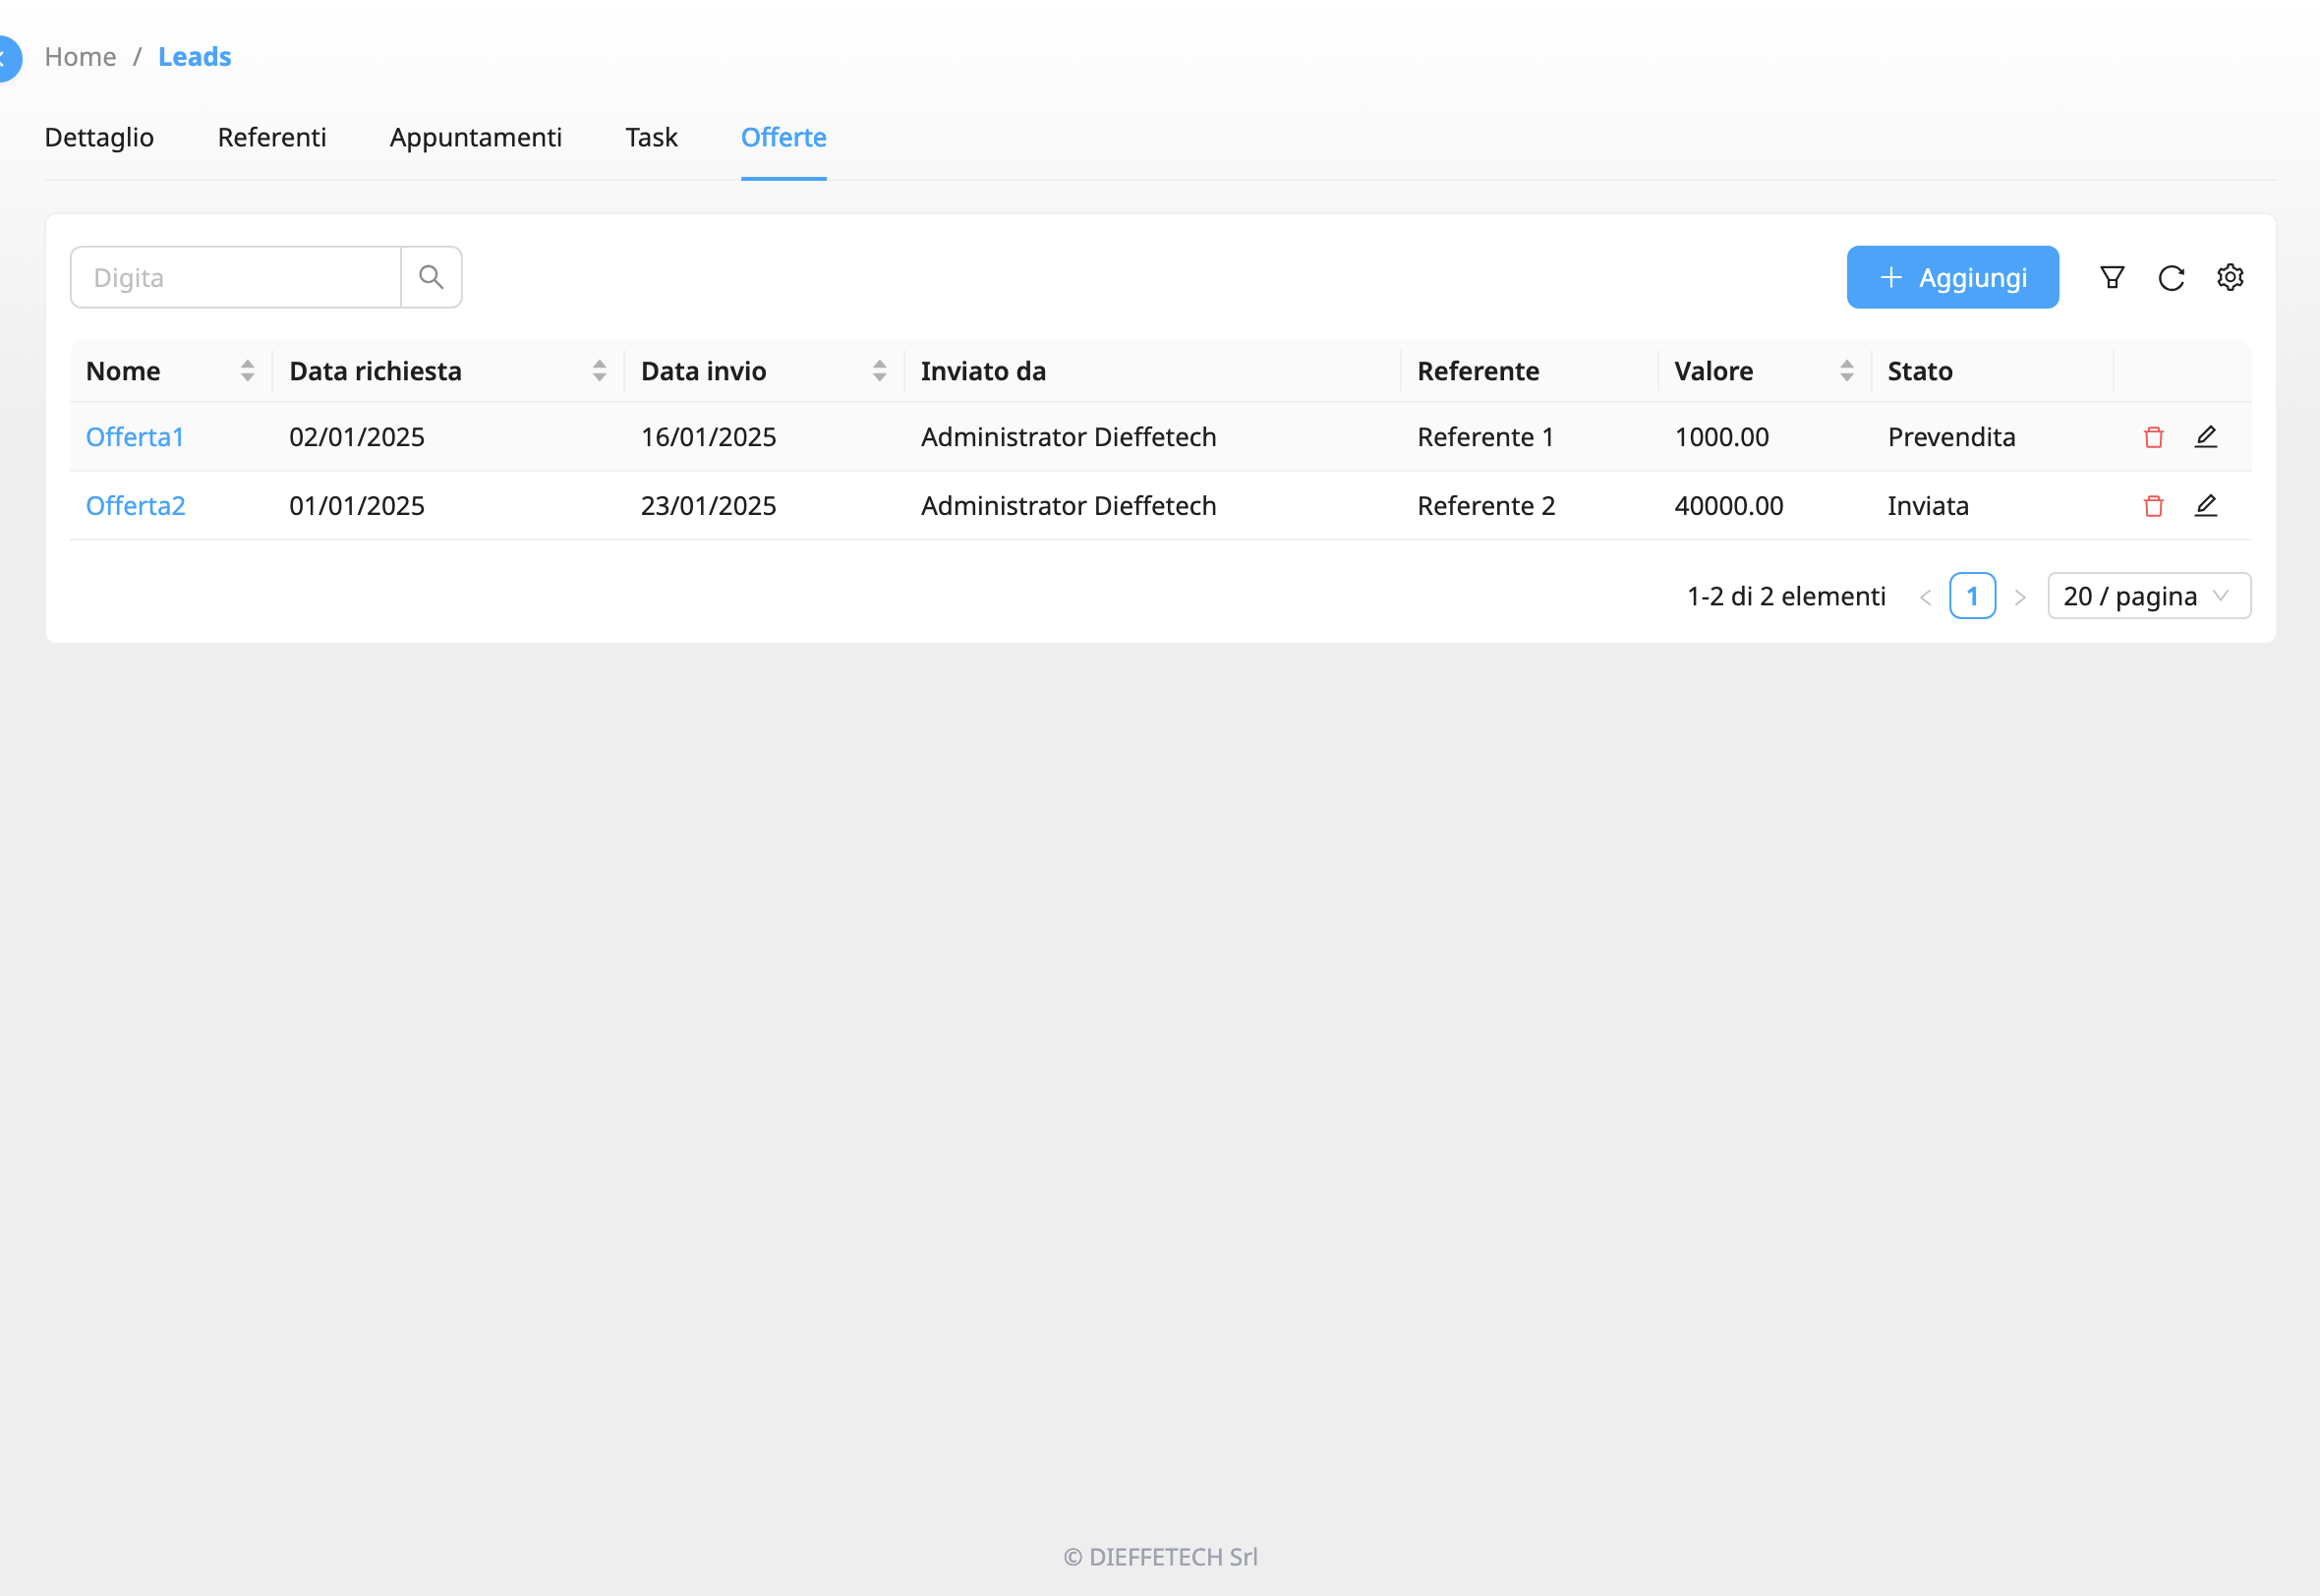
\includegraphics[width=1.0\textwidth]{immagini/OffersTableLeadsDetails.png}
    \caption{Tabella delle offerte.}
    \label{fig:offers_table}
\end{figure}

A prima vista, la tabella potrebbe sembrare simile alle altre, e in effetti, in termini di componenti, lo è. Si tratta infatti di una \textbf{CrudDataTable}, con il suo pulsante \textbf{+Aggiungi} che, al click, apre il form di inserimento.\pagebreak
\\Quando si accede ai dettagli di un’offerta (cliccando sull'icona della matita), si apre un form di modifica, visualizzato come un "drawer" (poiché viene aperto lateralmente), che consente di modificare i dettagli dell'offerta. Una funzionalità aggiuntiva in questa sezione è il pulsante \textbf{"Aggiungi Revisione"}.

\begin{figure}[ht]
    \centering
    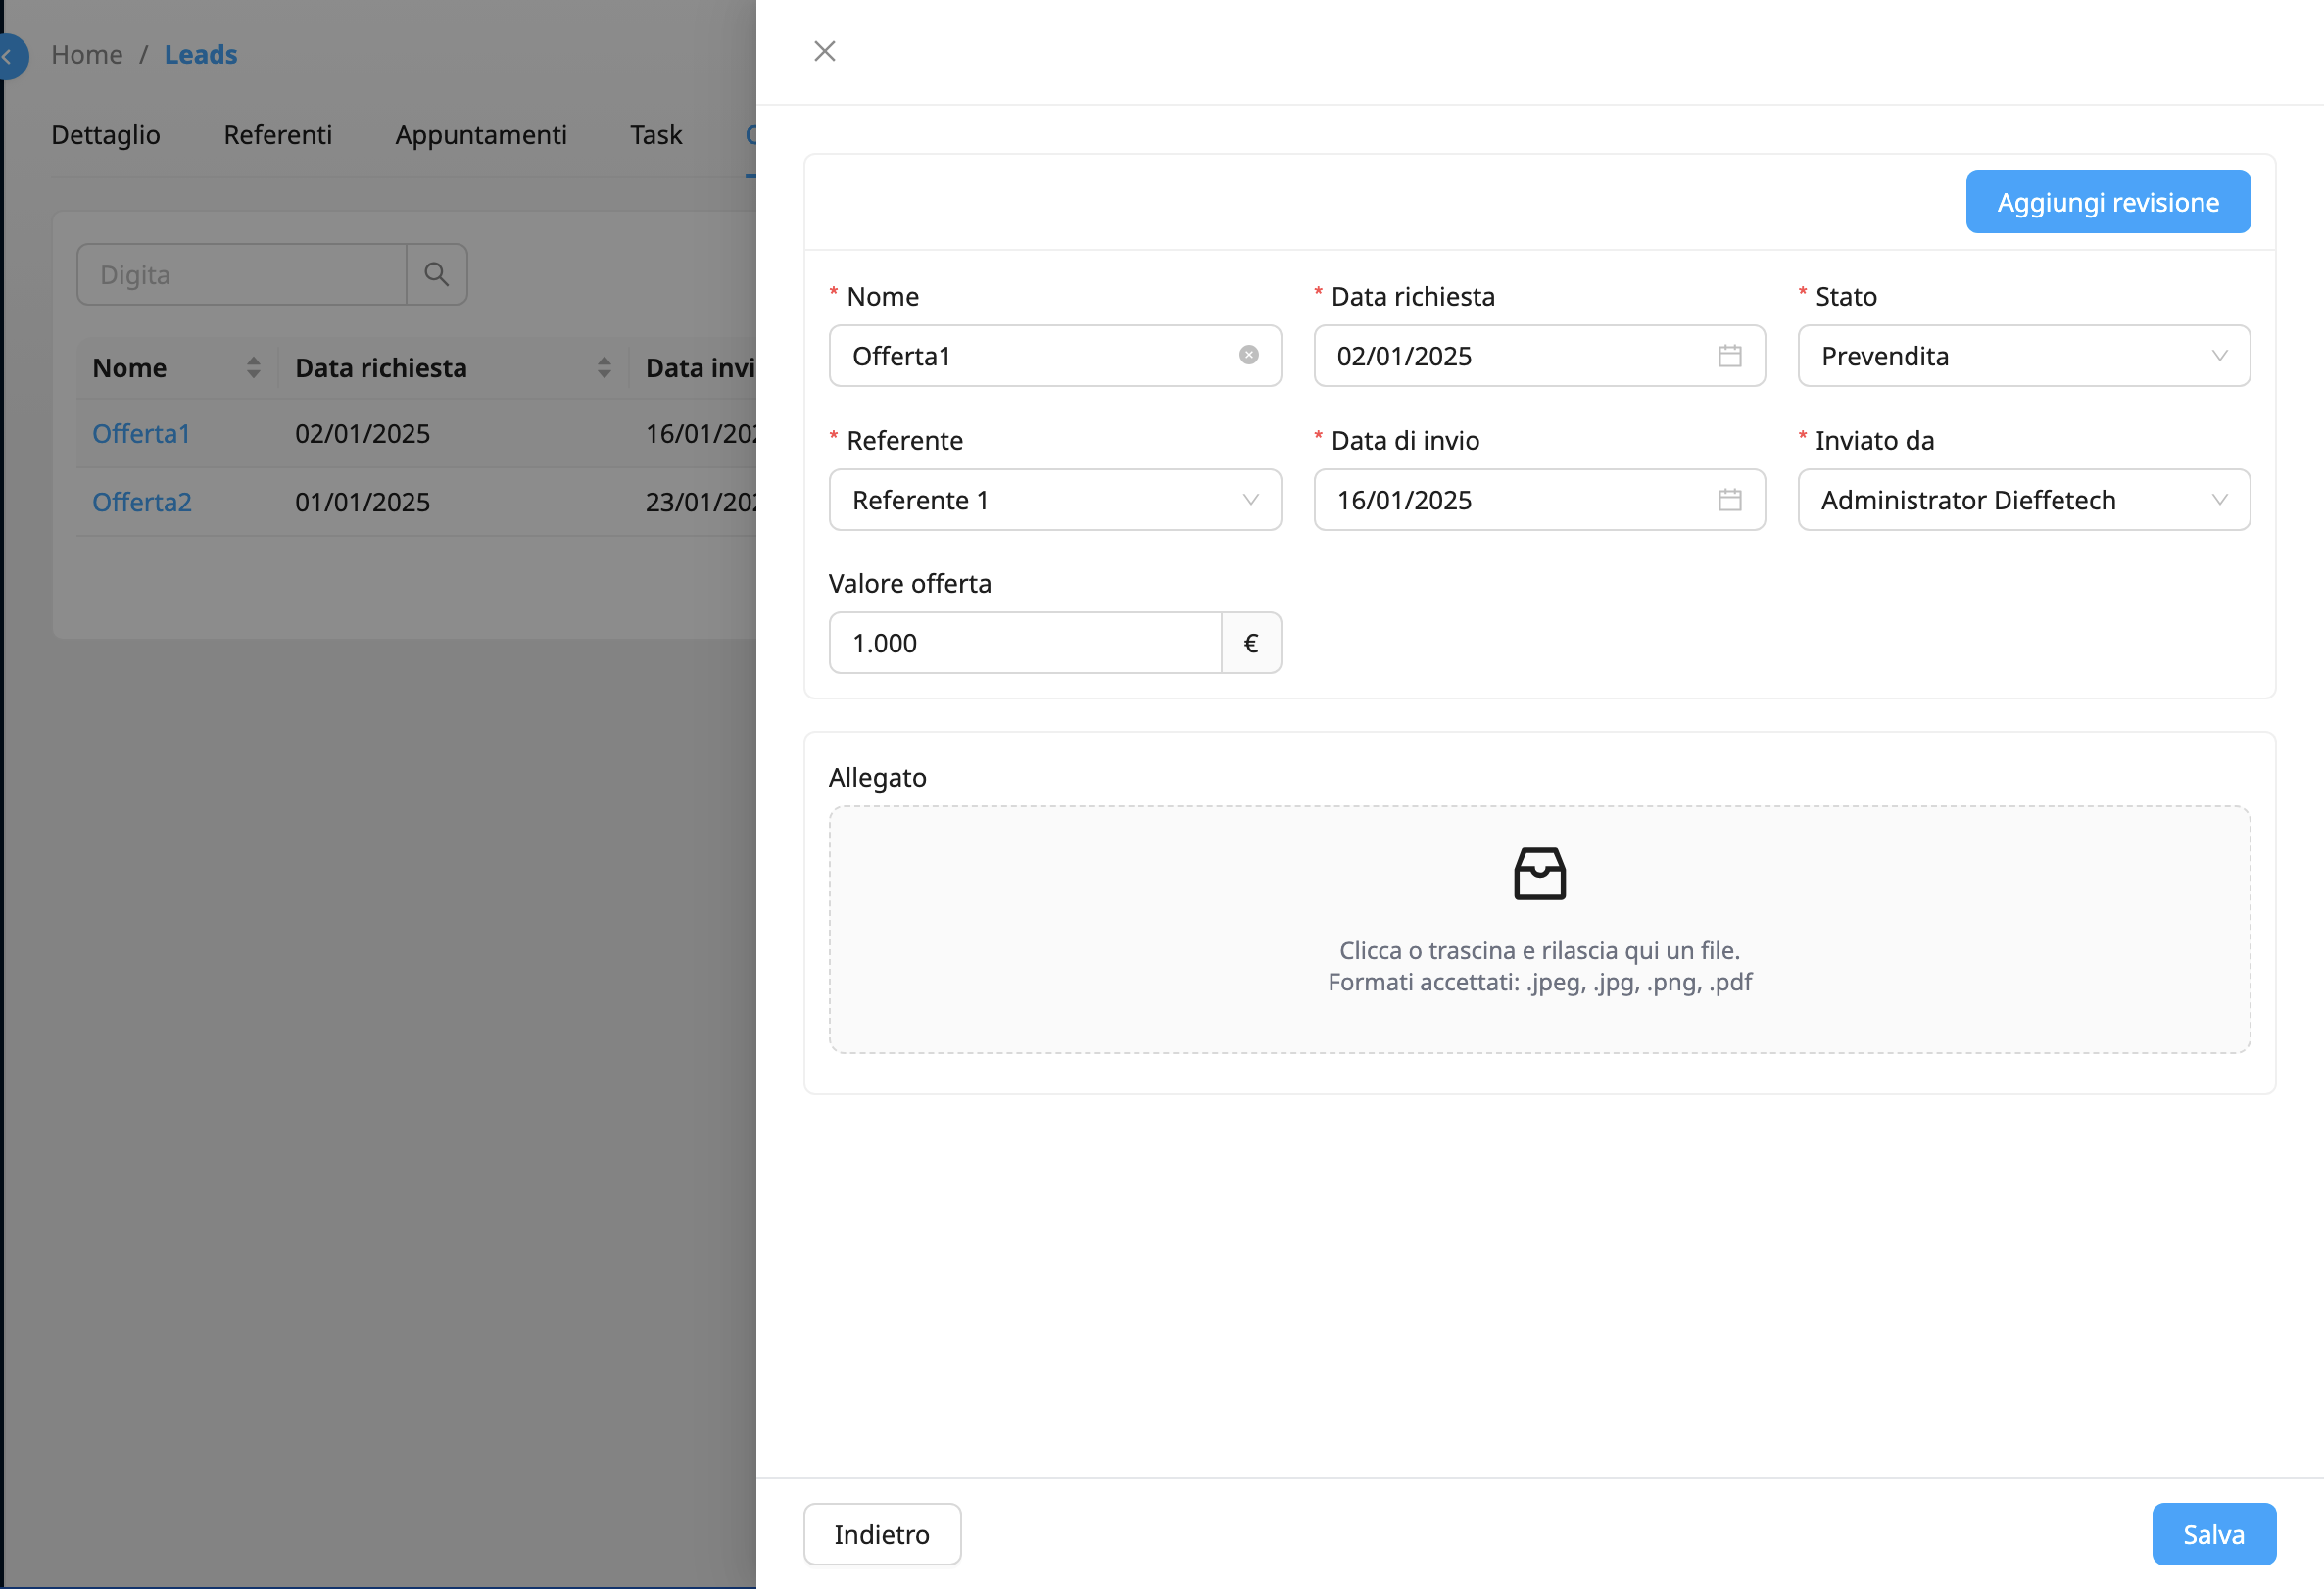
\includegraphics[width=0.7\textwidth]{immagini/OffersLeadsDetails.png}
    \caption{Dettaglio di un'offerta.}
    \label{fig:offers_details}
\end{figure}

Al clic, viene visualizzato un form aggiuntivo per la creazione di una revisione (di tipo "modal", in quanto ha il suo riquadro di compilazione in posizione centrale dello schermo). Una volta registrata, la revisione diventa un \textit{"children"} dell'offerta padre e viene visualizzata in tabella al posto dell'offerta originaria.

\begin{figure}[H]
    \centering
    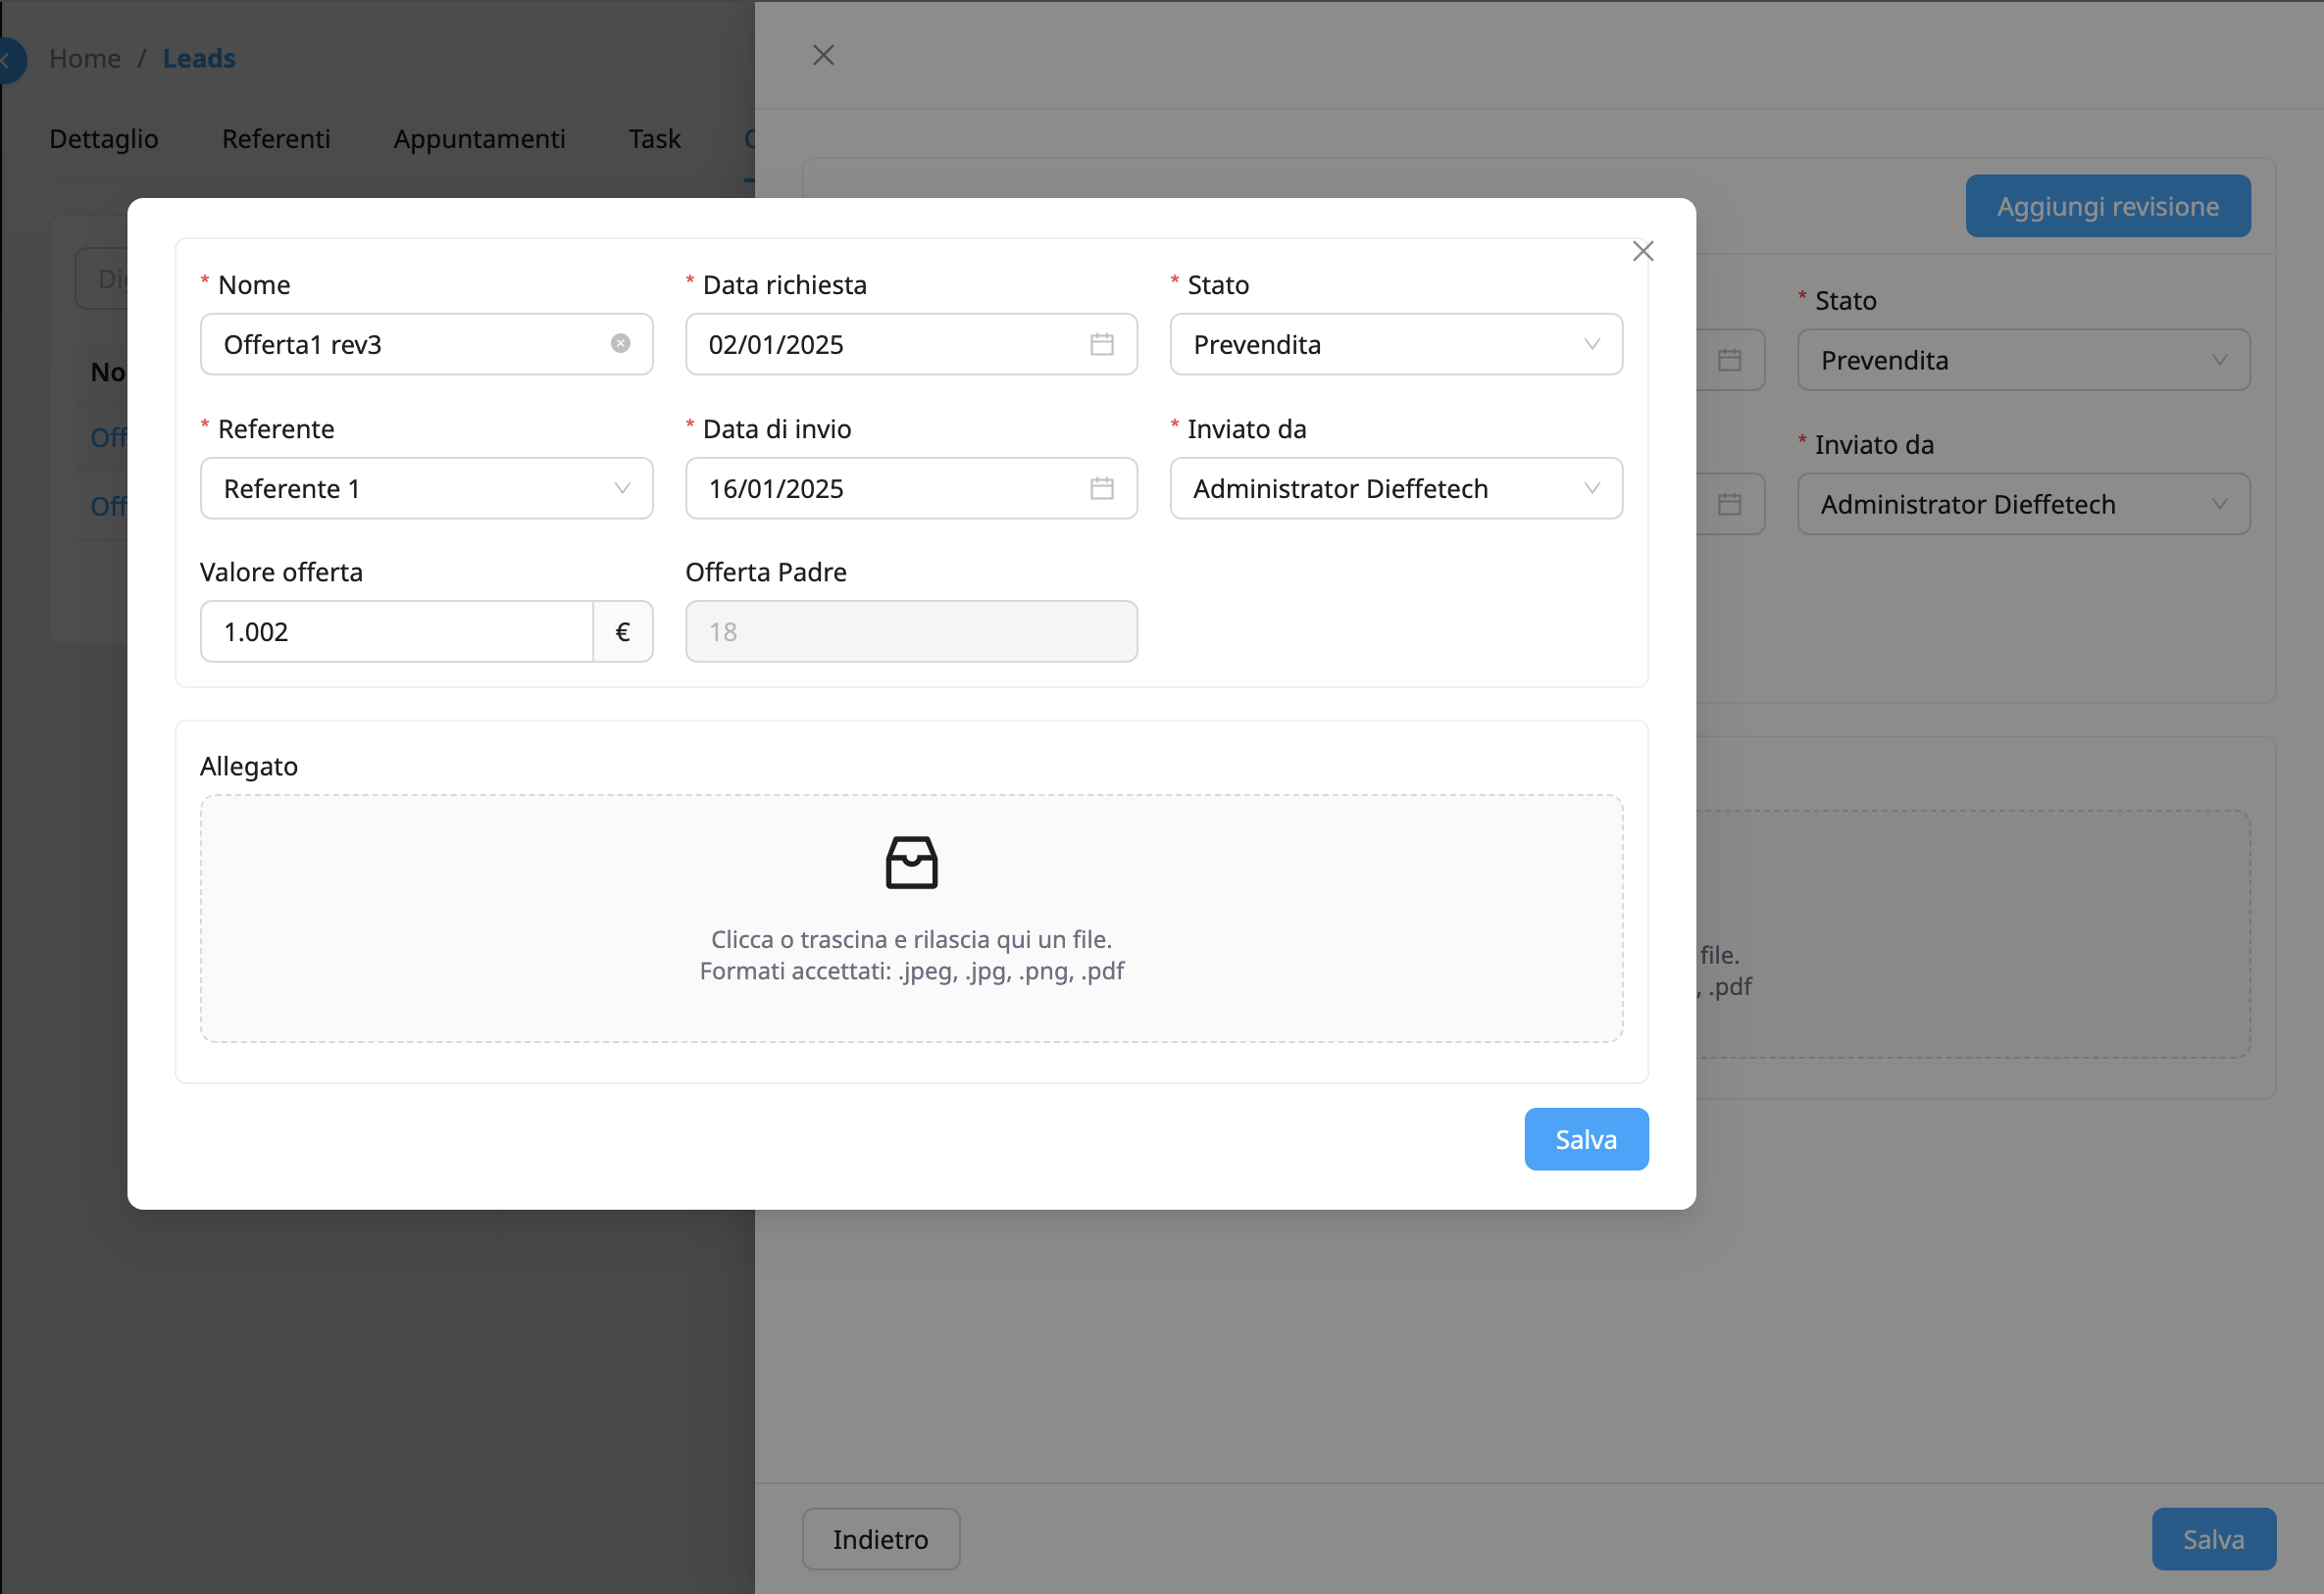
\includegraphics[width=0.7\textwidth]{immagini/RevisionForm.png}
    \caption{Modale di revisione.}
    \label{fig:revision_form}
\end{figure}

Cliccando sul nome dell’offerta, si accede alla pagina delle offerte, visualizzando i dettagli di quella selezionata. In questa vista, si possono notare due sezioni:
\begin{itemize}
    \item \textbf{Dettaglio}: il dettaglio dell'offerta selezionata.
    \item \textbf{Revisioni}: l'elenco di tutti gli stati precedenti dell'offerta, a partire dall'offerta iniziale fino a tutte le altre revisioni precedenti.
\end{itemize}

Nella sezione delle revisioni, avremo un elenco di tutti gli stati precedenti dell'offerta selezionata. Ponendo il caso di un'offerta con 3 revisioni, avremo l'offerta originale, la prima revisione e la seconda revisione.

\begin{figure}[H]
    \centering
    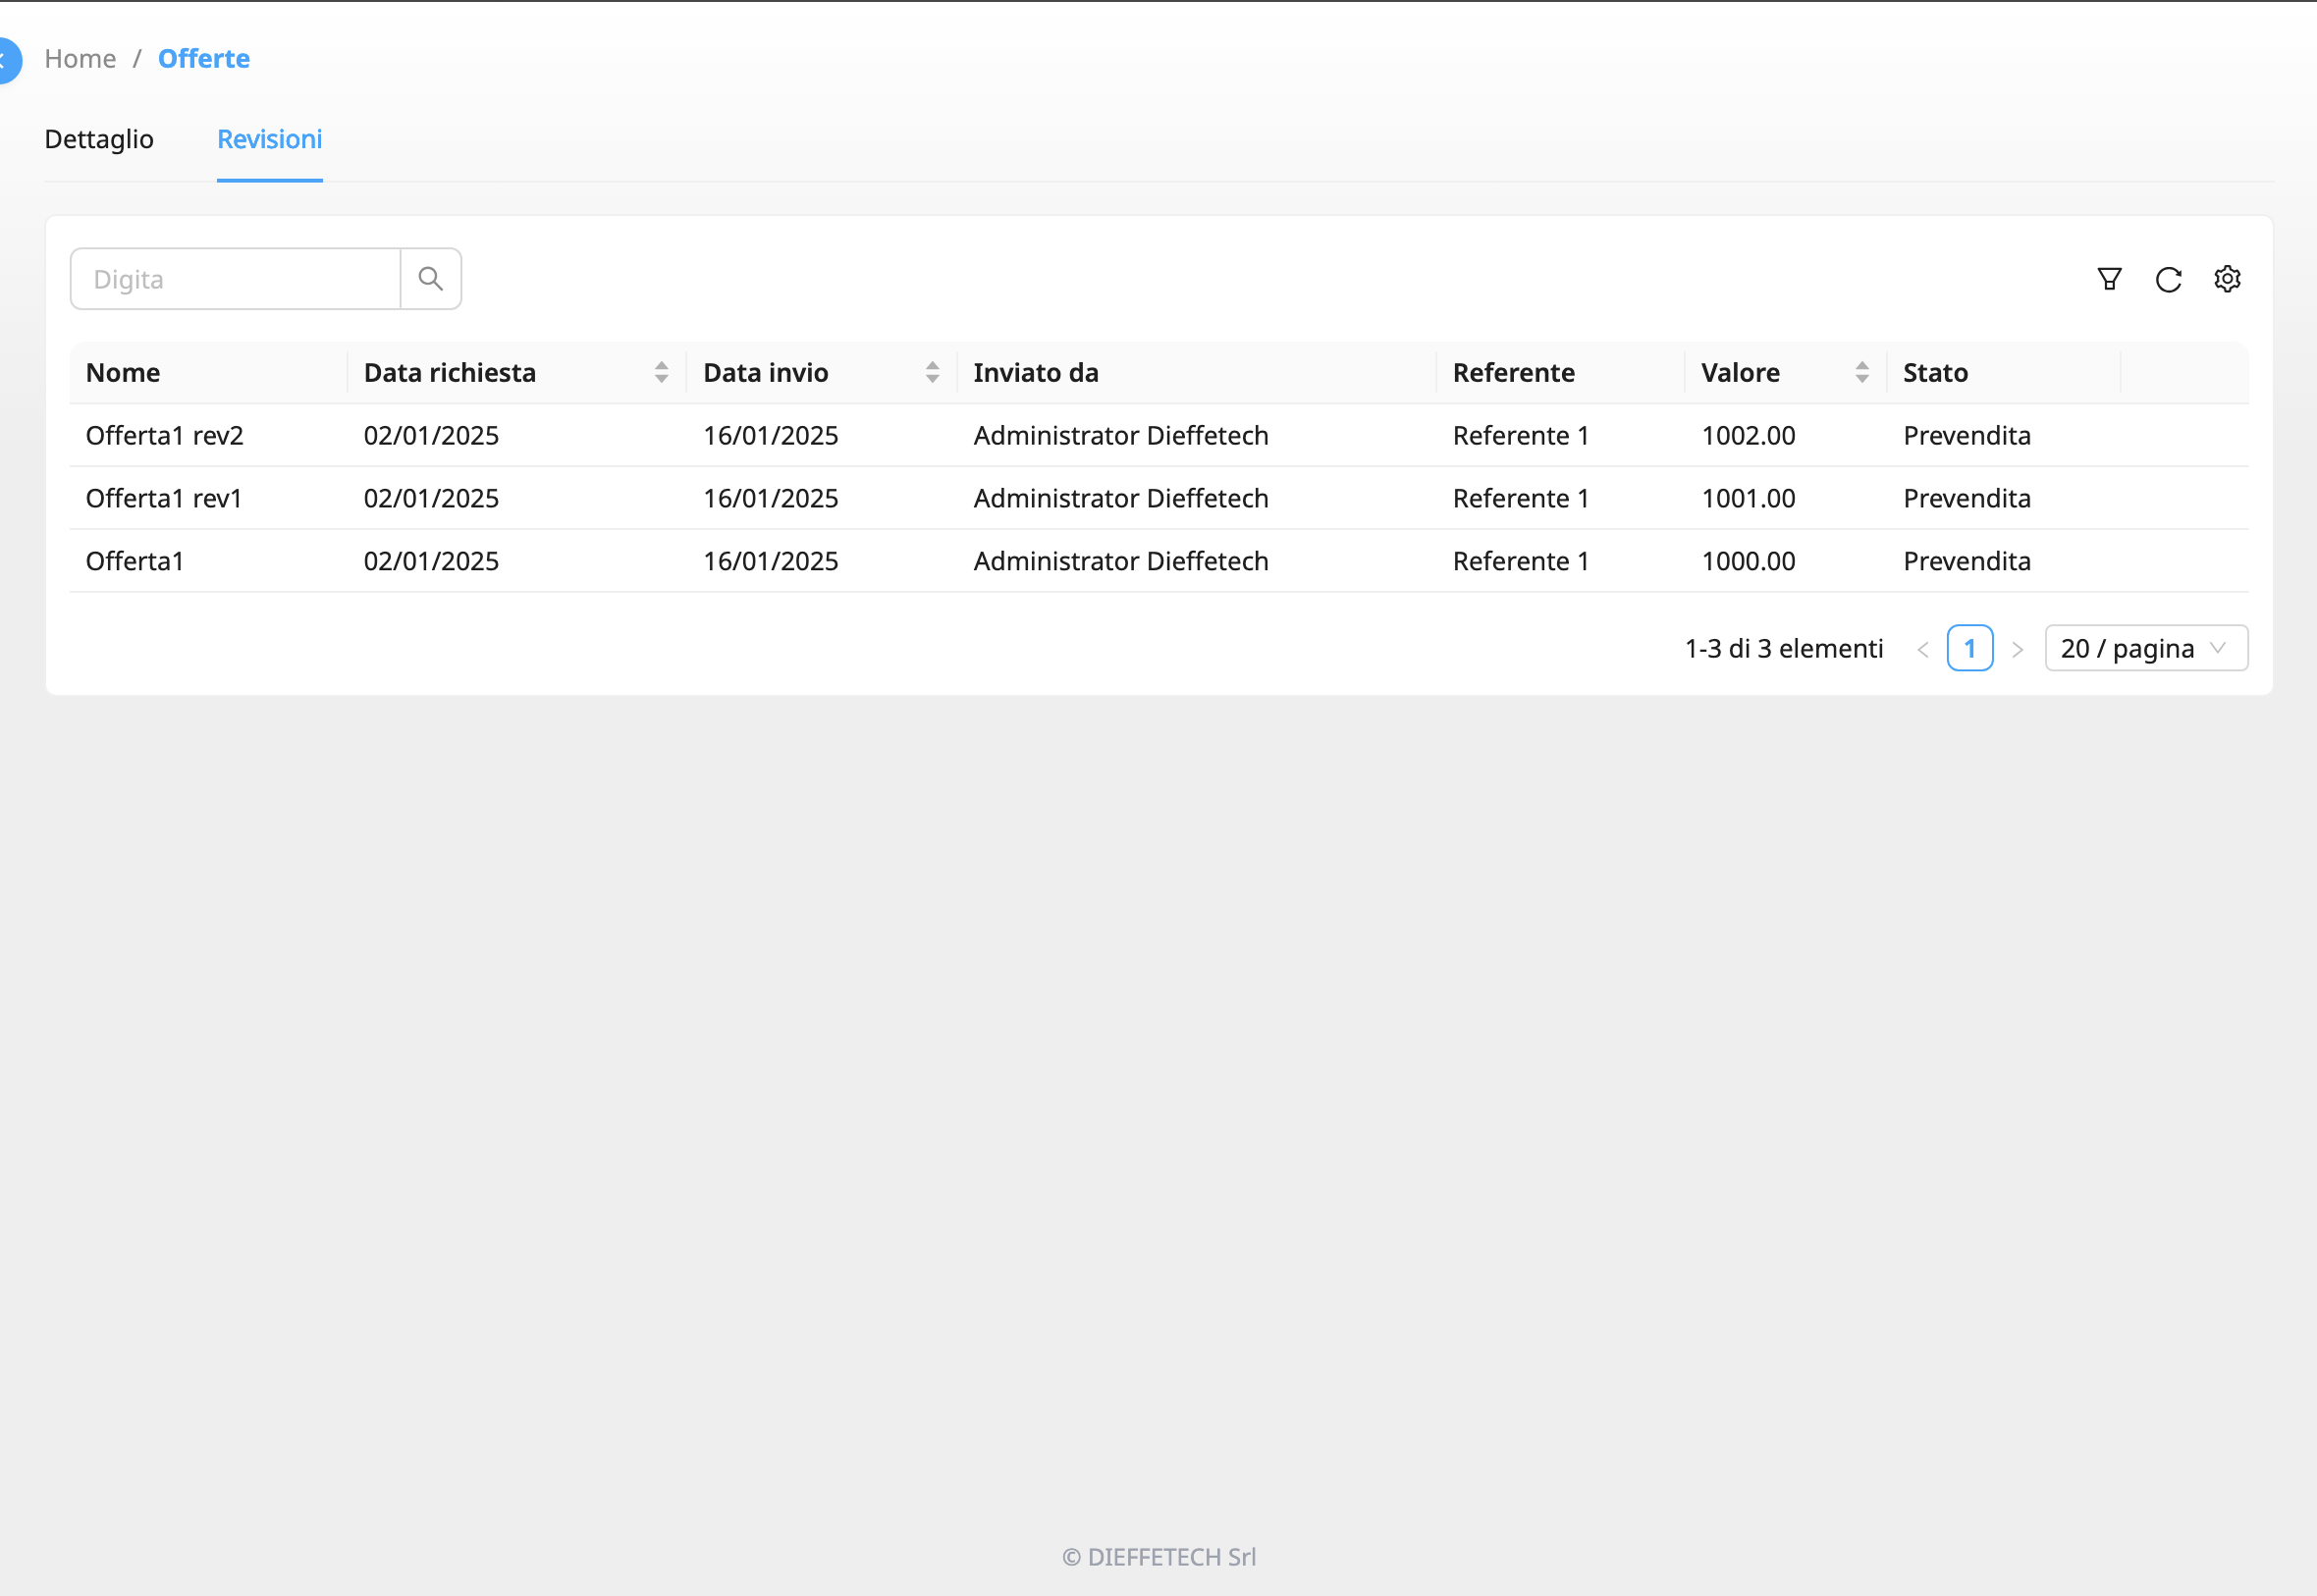
\includegraphics[width=1.0\textwidth]{immagini/OfferRevisions.png}
    \caption{Revisioni di un'offerta.}
    \label{fig:offer_revisions}
\end{figure}

\subsection{Offer Model}\label{sec:cap_sec_subsec_offer_model}
Per comprendere appieno i meccanismi di visualizzazione delle offerte e delle revisioni, è necessario analizzare il Model delle Offerte.
\begin{figure}[H]
\begin{multicols}{2}
\begin{lstlisting}[language=JavaScript, basicstyle=\scriptsize, numbers=none]
class Offer extends BaseModel
{
  use Log;

  protected $fillable = [
    'code',
    'name',
    'offer_value',
    ...
  ];

  protected $fillableMedia = [
    'attachment',
  ];

  protected $defaultSort = 'name';

  public function sortable(): array
  {
    return [
      'name',
      'offer_value',
      ...
    ];
  }

  public function filterable(): array
  {
    return [
      'name',
      'offer_value',
      AllowedFilter::callback('has_no_children', function ($query) {
        $query->whereNotIn('id', function ($subQuery) {
          $subQuery
            ->select('offer_parent_id')
            ->from('offers')
            ->whereNotNull('offer_parent_id');
        });
      }),
      ...
    ];
  }

  protected $searchable = [
      'name',
      ...
  ];
\end{lstlisting}
\break
\begin{lstlisting}[language=JavaScript, basicstyle=\scriptsize, numbers=none]
  // Relazioni
  public function customer(): BelongsTo
  {
    return $this->belongsTo(Customer::class)
  }

  public function userAdmin(): BelongsTo
  {
    return $this->belongsTo(UserAdmin::class)
  }

  public function referent(): BelongsTo
  {
    return $this->belongsTo(Referent::class)
  }

  public function parentOffer(): BelongsTo
  {
    return $this->belongsTo(Offer::class, 'offer_parent_id')->with('userAdmin', 'referent', 'parentOffer');
  }

  public function childrenOffer(): HasMany
  {
    return $this->hasMany(Offer::class, 'offer_parent_id')->with('userAdmin', 'referent', 'childrenOffer');
  }

  public function scopeHasNoChildren(Builder $query)
  {
    return $query->whereNotIn('id', function ($subQuery) {
      $subQuery
        ->select('offer_parent_id')
        ->from('offers')
        ->whereNotNull('offer_parent_id');
    });
  }
}
\end{lstlisting}
\end{multicols}
\caption{Model delle offerte}
\end{figure}
\break
Ogni Model ha una struttura generale con diverse sezioni per gestire le varie funzionalità dell'applicazione:\begin{itemize}
    \item \texttt{\$fillable}: Contiene tutti i campi del database che possono essere assegnati. Nel caso delle offerte, sono presenti tutti i campi necessari per rappresentare un'offerta nel database.
    
    \item \texttt{\$fillableMedia}: Gestisce gli allegati associati all'offerta, come file o media. Approfondiremo l'argomento nel capitolo \ref{sec:cap_sec_subsec_media}.

    \item \texttt{\$defaultSort}: Definisce la colonna di ordinamento predefinito per la visualizzazione delle offerte. Questo determina quale campo verrà usato per ordinare le offerte nella vista tabellare.

    \item \texttt{sortable()}: Restituisce le colonne che possono essere utilizzate per il riordinamento delle offerte. Consente una gestione dinamica dell'ordinamento attraverso il frontend, migliorando la flessibilità dell'interfaccia utente.

    \item \texttt{filterable()}: Definisce le colonne che possono essere filtrate dal frontend. Questa funzione include anche filtri avanzati come\\
    \texttt{AllowedFilter::callback()}, che ad esempio può escludere le offerte che hanno delle revisioni (offerte figlie).

    \item \texttt{\$searchable}: Elenca tutte le colonne del database che possono essere ricercate dal frontend. Permette una funzionalità di ricerca rapida e dinamica per gli utenti.

    \item \textbf{Funzioni di Relazione}:
    \begin{itemize}
        \item \texttt{customer()}: Definisce la relazione \texttt{BelongsTo} con il modello\\
        \texttt{Customer}. Rappresenta il legame tra l'offerta e il cliente a cui è associata, permettendo di accedere ai dettagli del cliente direttamente dal record dell'offerta.
        
        \item \texttt{userAdmin()}: Definisce la relazione \texttt{BelongsTo} con il modello\\
        \texttt{User}. Questa relazione indica quale amministratore ha gestito o creato l'offerta, fornendo una connessione diretta ai dati dell'utente responsabile.
    
        \item \texttt{referents()}: Definisce la relazione \texttt{BelongsTo} con il modello\\
        \texttt{Referent}. Indica quali referenti sono associati all'offerta, permettendo di accedere ai contatti all'interno dell'azienda cliente direttamente tramite l'offerta. Approfondiremo l'argomento nel capitolo \ref{sec:cap_sec_subsec_referenti}.
        
        \item \texttt{parentOffer()}: Definisce la relazione \texttt{BelongsTo} con l'offerta padre. Questa relazione è utile per gestire le offerte che sono delle revisioni o delle varianti di un'offerta precedente.
        
        \item \texttt{childrenOffer()}: Definisce la relazione \texttt{HasMany} per gestire tutte le revisioni di un'offerta. Le offerte figlie sono visualizzate in tabella al posto dell'offerta padre una volta che vengono create.
    \end{itemize}
    

    \item \textbf{Funzioni Scope}:
    \begin{itemize}
        \item \texttt{scopeHasNoChildren()}: Definisce uno scope per ottenere solo le offerte che non hanno revisioni associate. Viene utilizzato per filtrare e visualizzare nella tabella delle Offerte, solo le righe nel DB che non hanno nessun figlio associato, ovvero la revisione più recente.
    \end{itemize}

    \item \textbf{Funzioni Personalizzate}:
    \begin{itemize}
        \item \texttt{generateCode()}: Una funzione personalizzata che genera un codice unico per ogni offerta, basato sull'ID del cliente e sull'ID dell'offerta padre. Questo codice serve a identificare in modo univoco ogni offerta e le sue eventuali revisioni.
    \end{itemize}
\end{itemize}

\subsection{Children e Parents}\label{sec:cap_sec_subsec_children_parents}
Le relazioni \texttt{Children} e \texttt{Parent}  costituiscono relazioni ricorsive, in quanto entrambe sono definite all’interno del modello \texttt{Offer} e fanno riferimento alla medesima entità, ovvero l’offerta. Queste relazioni permettono di gestire la gerarchia tra le offerte e le loro revisioni.

\begin{itemize}
    \item \texttt{Children}: Questa relazione tiene traccia delle offerte figlie di un'offerta esistente. Quando un'offerta viene creata, essa non ha né genitori né figli. Tuttavia, alla creazione di una revisione, l'offerta originale diventa il "genitore" e la revisione diventa il "figlio". In questo modo, si forma una catena di revisioni, che collega l'offerta originale (il genitore) a tutte le sue revisioni successive (i figli).\\
    La catena si estende così: \textit{Offerta $\rightarrow$ Revisione1 $\rightarrow$ $\dots$ $\rightarrow$ RevisioneX}, con ogni revisione che punta alla precedente e viceversa.

    \item \texttt{Parent}: Questa relazione permette di risalire dalla revisione corrente all'offerta originale (il genitore). Tramite questa struttura, è possibile mantenere un collegamento tra l'offerta iniziale e la sua ultima revisione, che sarà quella visibile nella tabella principale delle offerte.

\end{itemize}

Grazie a queste relazioni "a catena", è possibile ottenere sia l'offerta iniziale che la sua ultima revisione, garantendo una navigazione fluida tra le varie versioni di un'offerta. Questa struttura è anche essenziale per la sezione "Revisioni" presente nei dettagli dell'offerta, poiché permette di risalire lungo la catena delle revisioni, dall'ultima fino all'offerta da cui tutto è iniziato.

Un'altra caratteristica interessante è l'utilizzo della funzione\\
\texttt{->with("attributi")}. Questa funzione assicura che, quando viene caricata un'offerta o una revisione (sia essa figlia o genitore), vengano caricati anche i relativi attributi e le rispettive relazioni. In questo modo, è possibile ottenere l'intera catena di relazioni \textit{genitore-figlio}, dall'offerta originale fino all'ultima revisione, con un solo caricamento, evitando il cosiddetto "N + 1 query problem".

\section{Morph Relations}

Le \textbf{morph relations} sono un tipo particolare di relazioni in Laravel che permettono a un singolo modello di appartenere a più altri modelli su una singola associazione. A differenza delle relazioni tradizionali, in cui un modello appartiene sempre a un altro modello specifico (es. una relazione \texttt{hasOne} o \texttt{belongsTo}), le morph relations consentono una maggiore flessibilità e riutilizzabilità.

Queste relazioni utilizzano una coppia di campi nel database: uno per memorizzare l'ID dell'entità collegata, e l'altro per memorizzare il tipo del modello. Questo significa che un modello può essere associato a diversi modelli di tipo differente tramite la stessa relazione. Un esempio semplice, un modello \texttt{Comment} potrebbe appartenere a modelli \texttt{Post} o \texttt{Video}, senza bisogno di creare relazioni distinte.

Esistono due tipi principali di relazioni morph:

\begin{itemize}
    \item \textbf{Relazione one-to-one} o \textbf{one-to-many morph}: permette a un modello di appartenere a uno o più modelli di tipo differente. Ad esempio, un commento può essere associato sia a un post che a un video.
    \item \textbf{Relazione many-to-many morph}: permette a un modello di appartenere a più modelli di tipo differente in una relazione many-to-many. Ad esempio, un tag può essere associato sia a post che a video.
\end{itemize}

Le morph relations sono estremamente utili per ridurre la duplicazione di codice e mantenere il database flessibile, specialmente quando si lavora con sistemi che richiedono l'associazione dinamica tra modelli di diversa natura.


\subsection{Referenti}\label{sec:cap_sec_subsec_referenti}

Ogni \textbf{Cliente} o \textbf{Lead} può avere più referenti, a ciascuno dei quali possono essere attribuiti più appuntamenti e offerte. Nella sezione \textit{Referenti}, verrà visualizzato un elenco dei referenti esistenti per il cliente selezionato, con la possibilità di aggiungerne di nuovi tramite il form accessibile cliccando sul bottone \texttt{+Aggiungi}.

\begin{figure}[H]
	\centering
	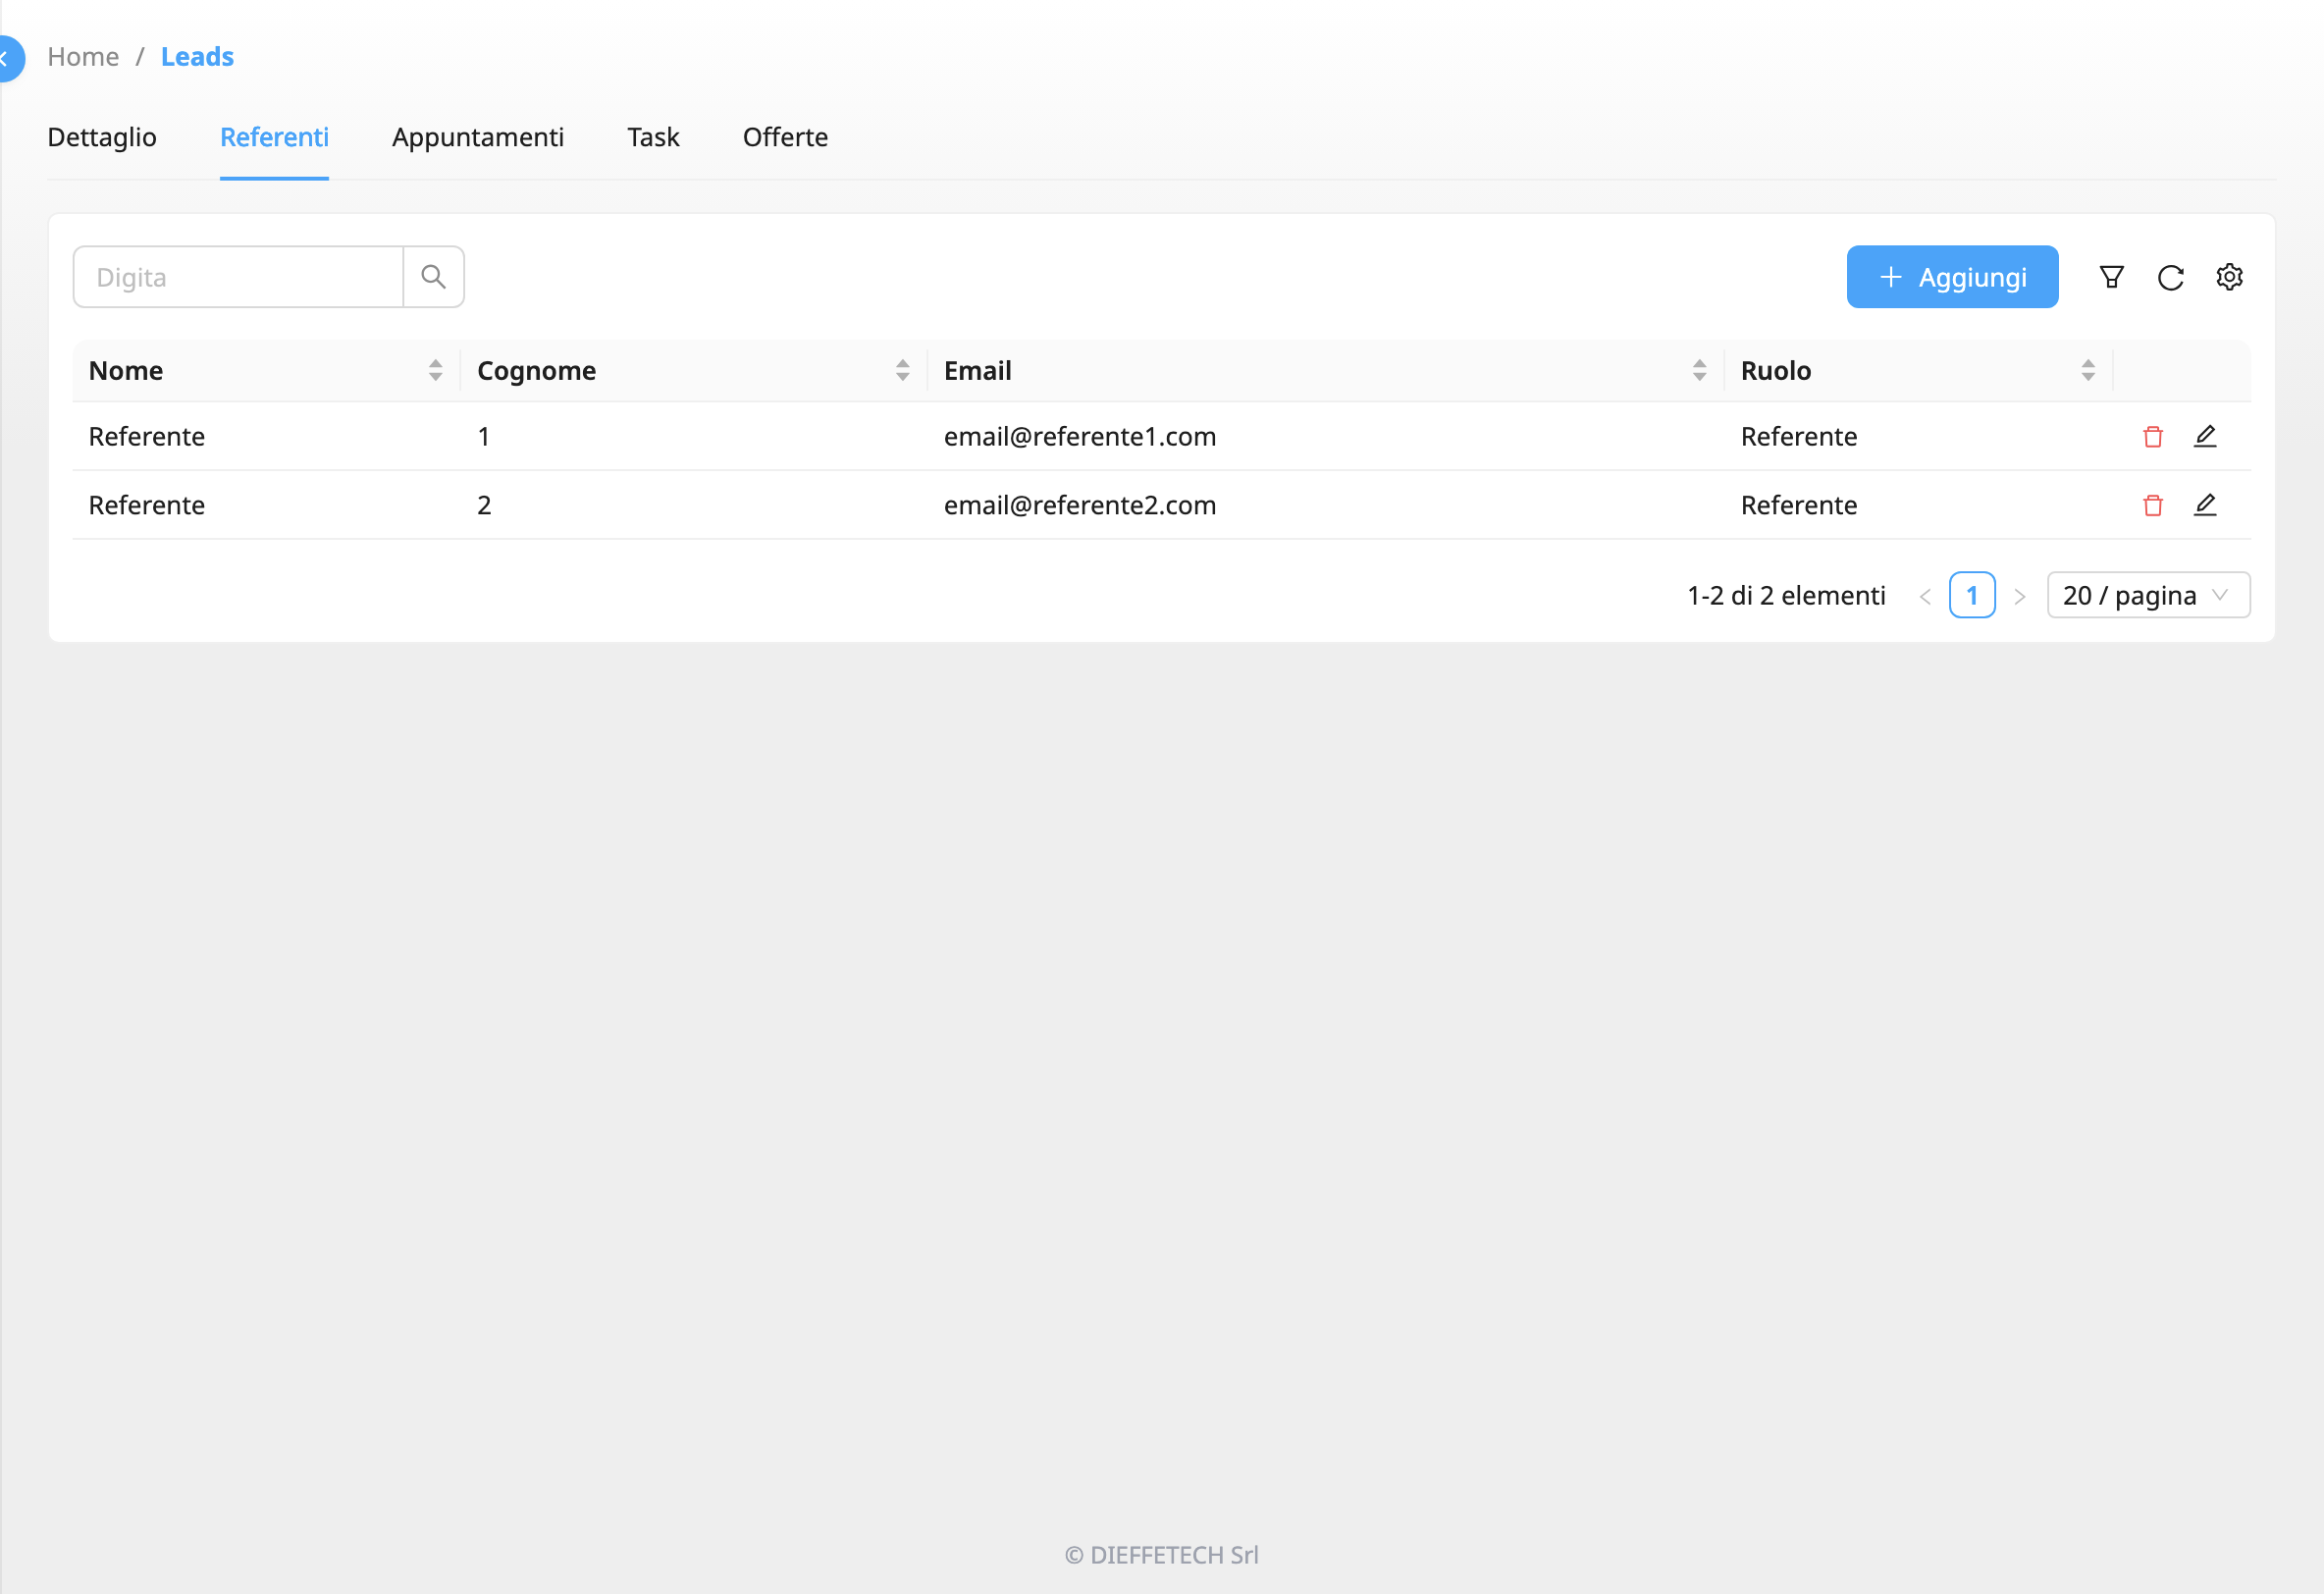
\includegraphics[width=1.0\textwidth]{immagini/RerefentTable.png}
	\caption{Tabella dei referenti.}
	\label{fig:referent_table}
\end{figure}

Ogni cliente ha i propri referenti, e infatti, durante la compilazione di un appuntamento, nell'elenco dei referenti disponibili ci saranno solo quelli associati al cliente o lead selezionato.\\\\\\\\\\\\
\begin{figure}[H]
	\centering
	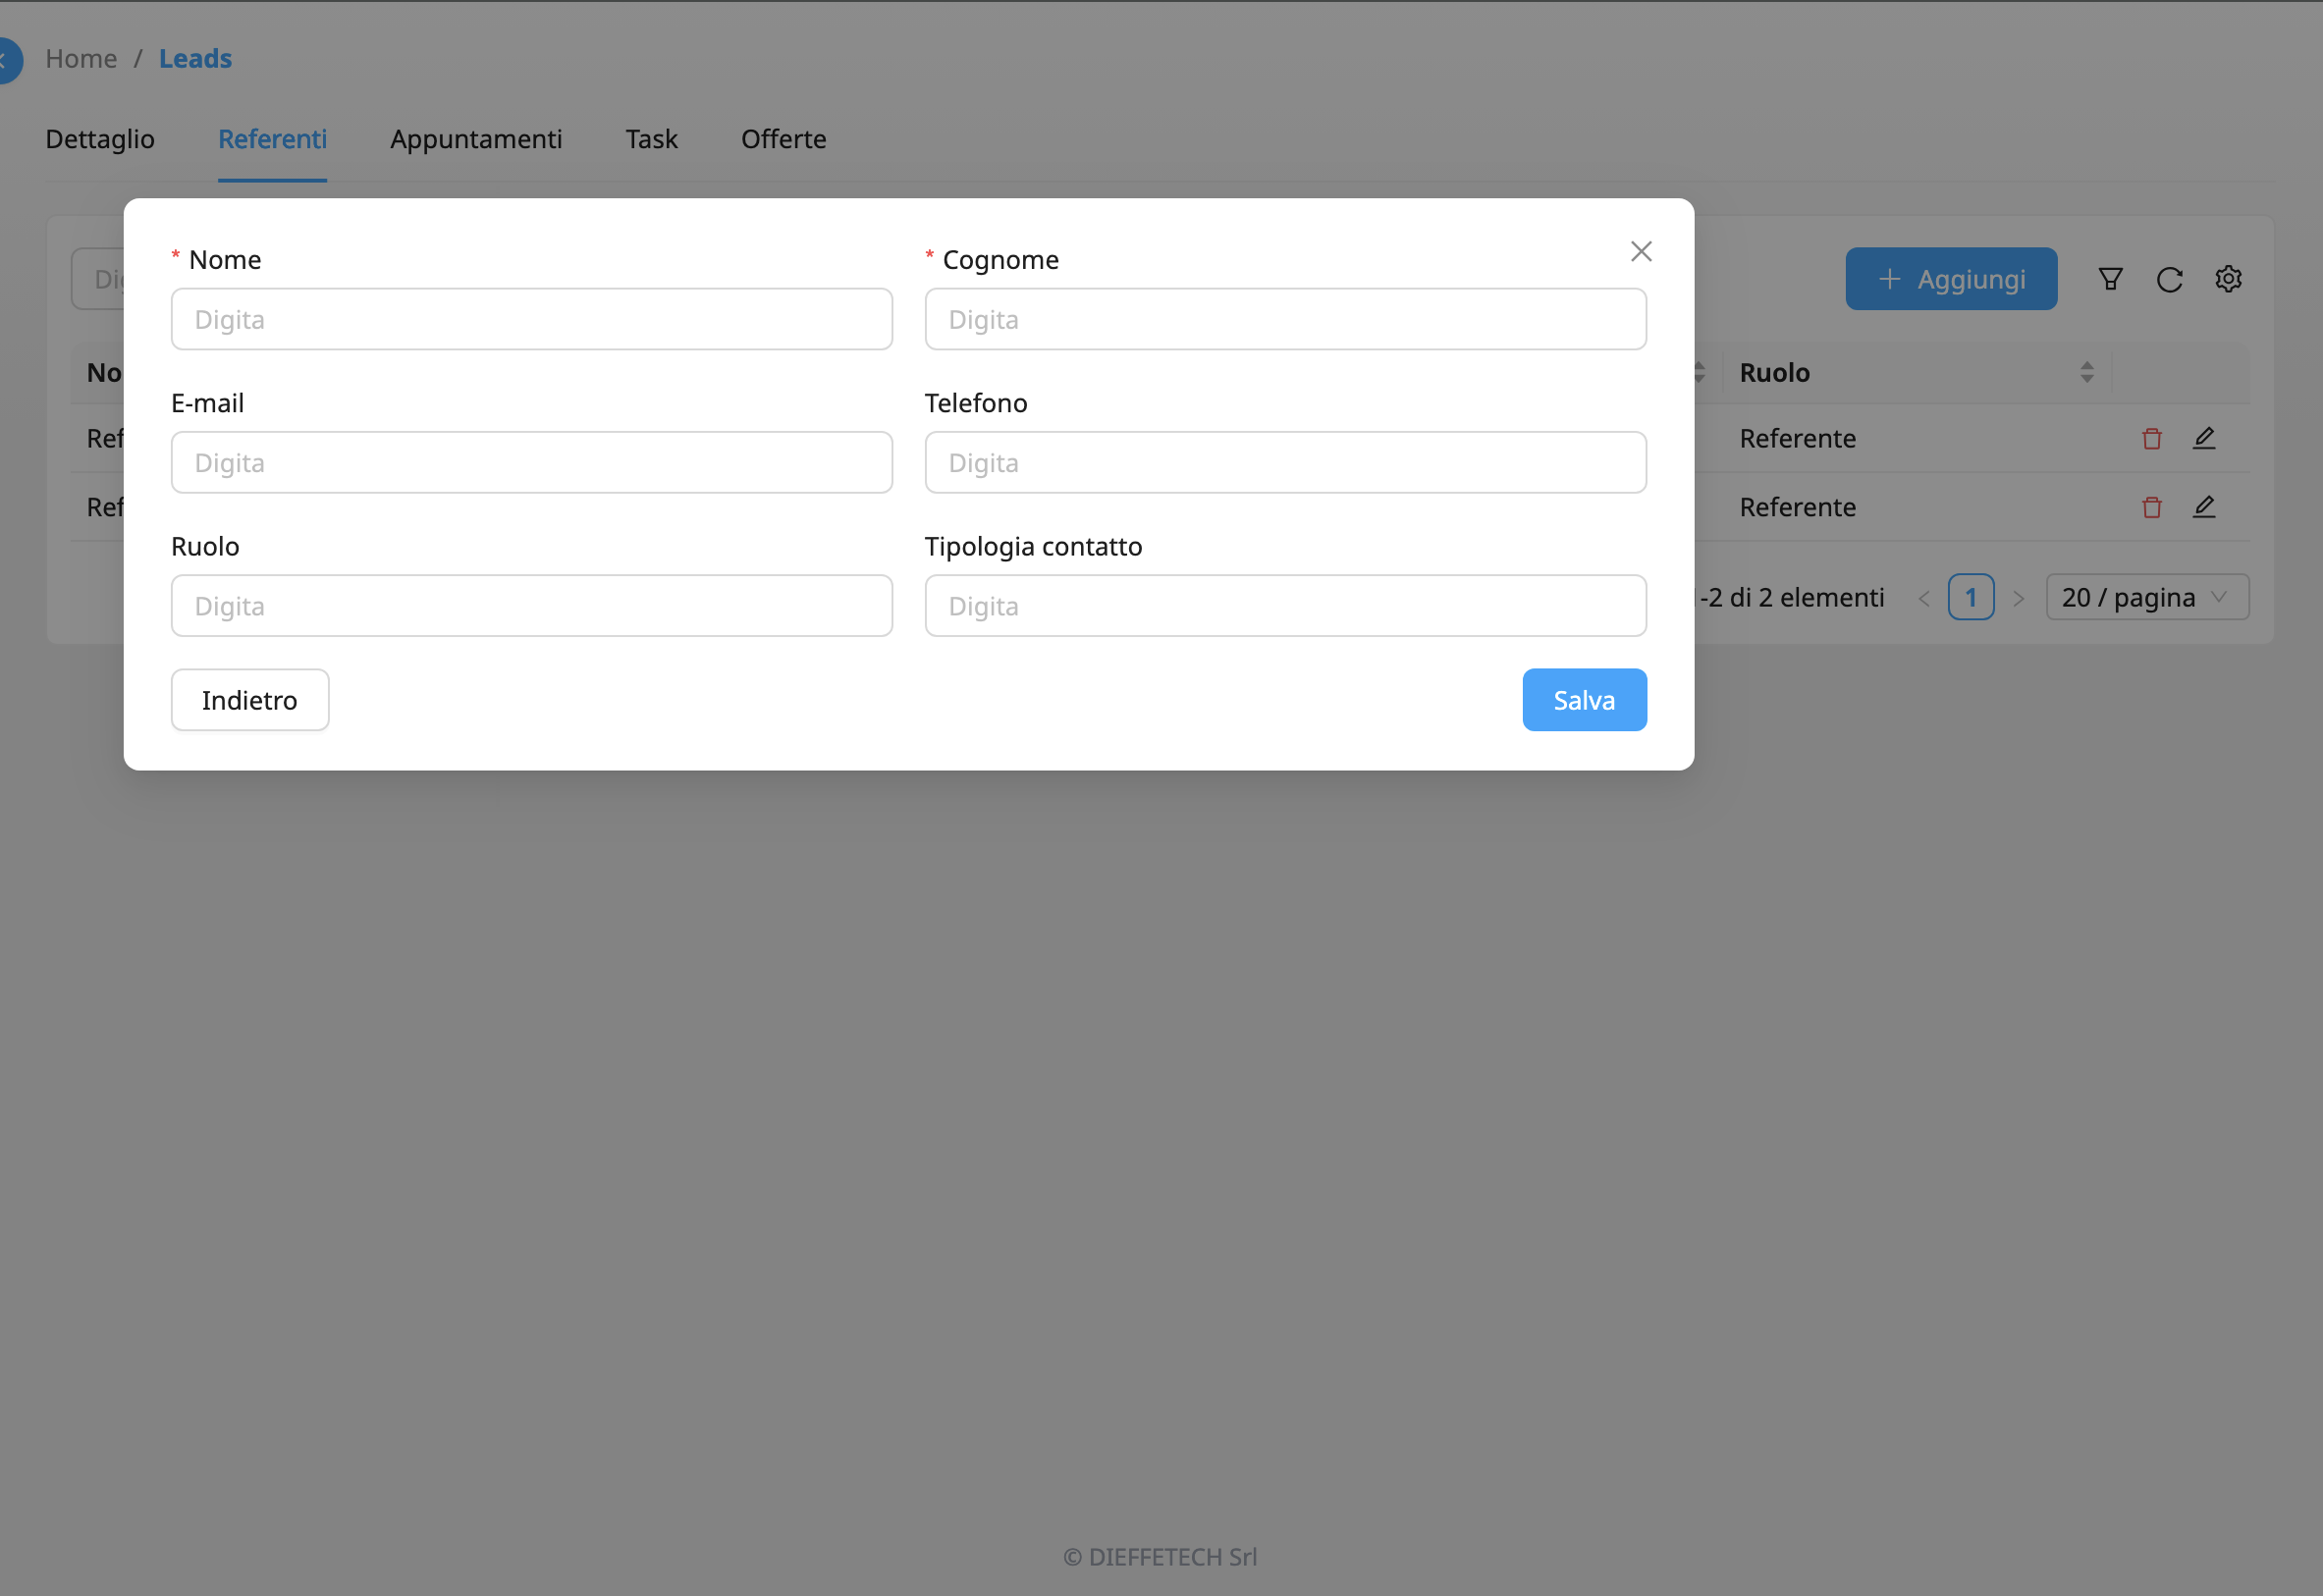
\includegraphics[width=1.0\textwidth]{immagini/ReferentForm.png}
	\caption{Form di inserimento per i referenti.}
	\label{fig:referent_form}
\end{figure}

L'aggiunta di un nuovo referente avviene tramite il relativo form, che permette di inserire i dati del referente. Il "collegamento" del referente al cliente avviene tramite la relazione morph. 

Una volta creato un nuovo referente, il database viene aggiornato con l'aggiunta di un record contenente i dati inseriti nel form. In particolare, le colonne \texttt{model\_type} e \texttt{model\_id} vengono automaticamente valorizzate in base alla posizione corrente. Nel caso specifico, dopo aver creato due referenti per il cliente con ID 26, sono stati inseriti due record con i dati del form, e automaticamente la colonna \texttt{model\_type} è stata valorizzata con \texttt{App/Models/Customer} e \texttt{model\_id} con il valore 26, che rappresenta l'ID del cliente.

\begin{figure}[ht]
	\centering
	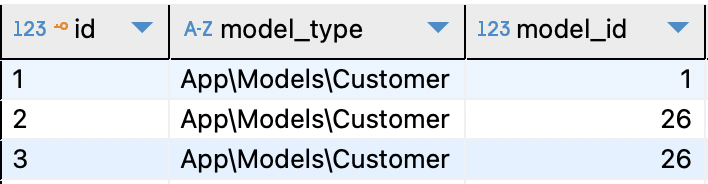
\includegraphics[width=1.0\textwidth]{immagini/ReferentDB.png}
	\caption{Referente nel database.}
	\label{fig:referent_db}
\end{figure}


\subsection{Media}\label{sec:cap_sec_subsec_media}
\sloppy
Nei form precedentemente discussi è presente una sezione denominata "allegati", che consente di caricare file immagine relativi all'appuntamento, all'offerta o al task selezionato.

La gestione dei file multimediali è affidata al componente \texttt{FilesUploader}.
\begin{lstlisting}[language=JavaScript, caption=Files Uploader, label=files_uploader, numbers=none]
    <FilesUploader
      storage="private"
      label={t("Allegati")}
      name={["attachment"]}
      uploadProps={{ listType: "picture-card}}
      multiple
      draggable
    />
\end{lstlisting}
Come la \texttt{CrudDataTable}, il \texttt{FilesUploader} dispone di alcune proprietà, tra cui:
\begin{itemize}
    \item \texttt{uploadProps}: Consente di configurare il tipo di anteprima per l'immagine caricata, con opzioni come \texttt{text}, \texttt{picture}, \texttt{picture-card} e \texttt{picture-circle}.
    \item \texttt{multiple}: Abilita o disabilita la possibilità di caricare più immagini contemporaneamente.
    \item \texttt{draggable}: Fornisce la funzionalità per riordinare manualmente le immagini caricate, permettendo all'utente di modificare l'ordine di visualizzazione.
\end{itemize}

I media, analogamente ai referenti, sono associati tramite una relazione \texttt{morph} definita nel loro modello, il che rende il componente altamente versatile e utilizzabile in qualsiasi altro modello all'interno del progetto.

Quando una foto viene aggiunta (prima di essere salvata), viene registrata automaticamente nel database come un record temporaneo, con \texttt{model\_type} impostato su un valore generico (\texttt{App/Models/Attachment}) e \texttt{model\_id} impostato su NULL.\\
\begin{figure}[H]
	\centering
	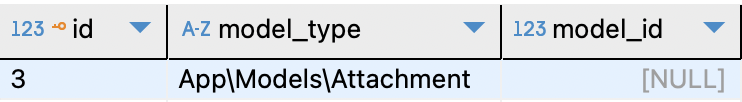
\includegraphics[width=1.0\textwidth]{immagini/MediaBefore.png}
	\caption{Media prima del salvataggio.}
	\label{fig:media_before}
\end{figure}
Questo record temporaneo viene mantenuto per un massimo di sette giorni. Se l'utente non conferma il salvataggio entro tale periodo, l'immagine viene eliminata automaticamente.

Quando l'utente salva l'immagine, grazie alla relazione \texttt{morph}, i campi \texttt{model\_type} e \texttt{model\_id} vengono automaticamente valorizzati. Per esempio, se ad un'offerta viene aggiunta un'immagine come allegato e successivamente salvata, in database verrà registrato un record con \texttt{model\_type} = \texttt{App/Models/Offer} e \texttt{model\_id} uguale all'ID dell'offerta (in questo caso, 19).
\begin{figure}[ht]
	\centering
	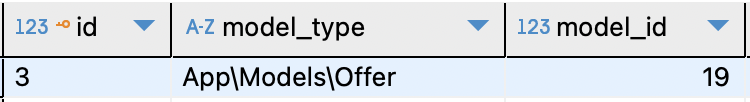
\includegraphics[width=1.0\textwidth]{immagini/MediaAfter.png}
	\caption{Media dopo il salvataggio.}
	\label{fig:media_after}
\end{figure}

Per garantire il corretto funzionamento dell'intero circuito di rilevamento dei modelli, è sufficiente aggiungere il campo \texttt{protected \$fillableMedia = ['attachment'];} all'interno del modello in cui si desidera gestire i media, in questo caso sia nel modello \texttt{Offer} che nei modelli \texttt{Appointment} e \texttt{Task}. Inoltre, è necessario inserire \texttt{->attachMediaFromRequest('attachment');} all'interno del controller, \texttt{OfferController}, nella sezione \texttt{store} o \texttt{update}.

\section{Scope Filters}\label{sec:cap_sec_subsec_scope_filters}
Oltre a filtrare per le colonne della tabella, è possibile dichiarare dei filtri personalizzati in base alle proprie esigenze. All'interno del Model delle Offerte, ad esempio, abbiamo un filtro \texttt{has\_no\_children} definito come segue:

\begin{lstlisting}[language=JavaScript, numbers=none]
AllowedFilter::callback('has_no_children', function ($query) {
  $query->whereNotIn('id', function ($subQuery) {
    $subQuery
      ->select('offer_parent_id')
      ->from('offers')
      ->whereNotNull('offer_parent_id');
  });
}),
\end{lstlisting}

Per ogni filtro personalizzato, ci deve essere la sua funzione annessa. In questo caso, filtrando per \texttt{has\_no\_children}, avremo all'interno del model una funzione:

\begin{lstlisting}[language=JavaScript, numbers=none]
public function scopeHasNoChildren(Builder $query)
{
  return $query->whereNotIn('id', function($subQuery) {
    $subQuery
      ->select('offer_parent_id')
      ->from('offers')
      ->whereNotNull('offer_parent_id');
  });
}
\end{lstlisting}

In questo caso, questa funzione è stata progettata per essere utilizzata nelle tabelle delle Offerte, al fine di visualizzare esclusivamente l'ultima revisione di ogni offerta, poiché sarà l'unica priva di un'offerta figlia.

\section{Offerta Accettata}\label{sec:cap_sec_subsec_accepted_offer}
Quando viene creata un'offerta, essa può trovarsi in uno dei seguenti quattro stati: \texttt{Prevendita}, \texttt{Inviata}, \texttt{Accettata} e \texttt{Rifiutata}. Inizialmente, l'offerta è impostata come \texttt{Prevendita}, ma se vengono effettuate delle revisioni e successivamente viene raggiunto un accordo, lo stato cambierà in \texttt{Accettata}. 

Al momento del salvataggio, se lo stato selezionato è \texttt{Accettata}, viene mostrata una modale di conferma.

Ogni form è avvolto dal componente \texttt{DfProForm}. Questo componente, simile ai componenti \texttt{CrudDataTable} e \texttt{FilesUploader}, dispone di alcune proprie \texttt{props}. Nel caso specifico di \texttt{DfProForm}, per fare in modo che la modale di conferma venga visualizzata solo quando lo stato è "Accettato", è sufficiente aggiungere la \texttt{prop} \texttt{withConfirmModal={status === "accepted"}}. Ulteriori dettagli, come il titolo, il contenuto e la larghezza della modale, sono configurabili tramite la \texttt{prop} \texttt{confirmModalProps}, che può includere un oggetto del tipo: \texttt{{title: "Titolo", content: "Contenuto", width: 400, type: "warn"}}.

Una volta confermata la modifica, i campi dell'offerta diventano non modificabili e viene avviato automaticamente un progetto relativo a quell'azienda. 

Questo comporta due situazioni:
\begin{itemize}
    \item Se l'offerta accettata è di un cliente, l'offerta verrà aggiornata e il progetto verrà creato correttamente.
    \item Se l'offerta accettata è di un lead, quest'ultimo verrà convertito in cliente, dopodichè l'offerta verrà aggiornata e il progetto verrà creato.
\end{itemize}
Il tutto è gestito all'interno del controller, nelle funzioni \texttt{store} e \texttt{update}.

\begin{lstlisting}[language=JavaScript, numbers=none, label=OfferController, caption=OfferController]
public function store(OfferRequest $request, Customer $customer)
{
    $data = $request->safe()->all();
    $parentId = isset($data['offer_parent_id']) ? $data['offer_parent_id'] : null;

    if ($data['status'] === 'accepted' && $customer->getAttributes()['is_customer'] === 0) {
        $customer['is_customer'] = 1;
        $customer->update([$customer]);
    }

    $code = Offer::generateCode($customer->id, $parentId);
    $data['code'] = $code;

    if($customer) {
        $offer = $customer->offers()->create($data);
    } else {
        return response()->json(['error' => 'Invalid request'], 400);
    }
    $offer->attachMediaFromRequest('attachment');
    return new OfferResource($offer);
}

public function update(OfferRequest $request, ?Customer $customer = null, Offer $offer)
{
  $data = $request->safe()->all();
  $offer->update($data);
  $offer->attachMediaFromRequest('attachment');

  if ($data['status'] === 'accepted' && $customer->getAttributes()['is_customer'] === 0) {
    $customer['is_customer'] = 1;
    $customer->update([$customer]);
  }
  return new OfferResource($offer);
}
\end{lstlisting}
\begin{itemize}
    \item \textbf{Metodo \texttt{store}:} 
    \begin{itemize}
        \item I dati inviati dal form vengono recuperati tramite \texttt{\$request->safe()->all()} e archiviati nella variabile \texttt{\$data}.
        \item Se presente, l'ID di un'offerta genitore (\texttt{offer\_parent\_id}) viene estratto e salvato in \texttt{\$parentId}, altrimenti viene impostato su \texttt{null}.
        \item Se lo stato dell'offerta è "accepted" (accettata) e il cliente non è ancora stato contrassegnato come cliente (\texttt{is\_customer} è 0), il campo \texttt{is\_customer} del cliente viene aggiornato a 1.
        \item Viene generato un codice univoco per l'offerta utilizzando il metodo \texttt{generateCode} del modello \texttt{Offer}, che prende come parametri l'ID del cliente e l'eventuale ID dell'offerta genitore.
        \item Se il cliente è valido, l'offerta viene creata e associata al cliente utilizzando la relazione \texttt{offers()} e i dati elaborati.
        \item Se sono presenti allegati, questi vengono associati all'offerta tramite il metodo \texttt{attachMediaFromRequest('attachment')}.
    \end{itemize}
    Al termine, viene restituita una risposta con l'oggetto \texttt{OfferResource}, che contiene i dettagli dell'offerta appena creata.

    \item \textbf{Metodo \texttt{update}:}
    \begin{itemize}
        \item I dati inviati nel form di aggiornamento vengono estratti e archiviati nella variabile \texttt{\$data}.
        \item L'offerta esistente viene aggiornata con i nuovi dati tramite il metodo \texttt{update()}.
        \item Se sono presenti allegati, questi vengono associati all'offerta tramite il metodo \texttt{attachMediaFromRequest('attachment')}.
        \item Se lo stato dell'offerta è "accepted" e il cliente non è ancora segnato come cliente (\texttt{is\_customer} è 0), il campo \texttt{is\_customer} viene aggiornato a 1.
    \end{itemize}
    Anche in questo caso, il metodo restituisce un oggetto \texttt{OfferResource}, che contiene i dettagli dell'offerta aggiornata.
\end{itemize}
